%!TEX root = ../../dissertation.tex
%%%%%%%%%%%%%%%%%%%%%%%%%%%%%%%%%%%%%%%%%%%%%%%%%%%%%%%%%%%%%%%%%%%%%%%%%%%%%%%%
\chapter{Video Streaming Techniques}
\label{chap:streaming}


%%%%%%%%%%%%%%%%%%%%%%%%%%%%%%%%%%%%%%%%%%%%%%%%%%%%%%%%%%%%%%%%%%%%%%%%%%%%%%%%
\section{Streaming Control Flow Nomenclature}


\begin{figure}[htbp]
\centering
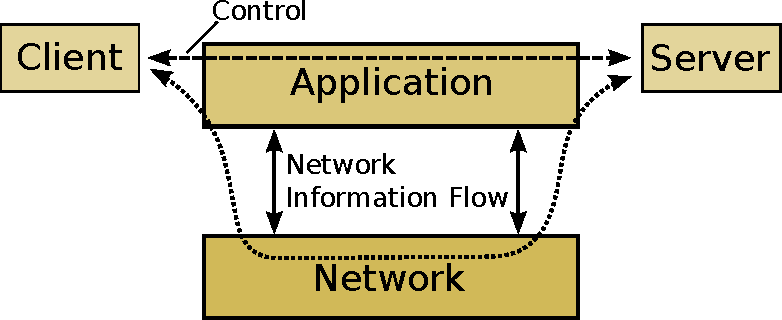
\includegraphics[width=0.8\textwidth]{images/nif.pdf}
\caption{Theoretical information exchange paths between streaming partners.}
\label{c3:fig:nif}
\end{figure}

In every network architecture there is a control information flow between its participating layers, protocols and elements (cf. also Fig. \ref{c3:fig:nif}). Control information may need to be exchanged to coordinate and negotiate the modes of communication between two endpoints and can be helpful in many ways. For example can a network explicitly expose network's quality of service data to applications or these application can make reservation requests to the network. Communication can also work implicitly, demonstrated in the distributed TCP congestion control enabled by the lack of resource isolation. This shows two major ways for the information flow to be implemented: Either through directly and explicitly exchanging information or by one participant implicitly drawing conclusions on another participants resources and behavior.

These different approaches can also be observed in video streaming. The explicit control structure of protocol suites like IMS\cite{3gpp.23.228} and MBMS weaves application and network layer tightly together. This theoretically allows for an improved streaming performance at the cost of universally applicable behavior. Today's IP-based HTTP streaming forms the other side of the pole having only an implicit network information flow by guessing the current network conditions.

For the future there are open questions on how to best incorporate this information flow into streaming applications. Of special interest is the kind of information an application should rely on, and which information the application really requires. Moreover, it is to be decided what and how information should flow in the network. To support the decision making, models and ways to evaluate and compare protocols and network architectures need to be thought out, possibly resulting in a generic evaluation model.





%%%%%%%%%%%%%%%%%%%%%%%%%%%%%%%%%%%%%%%%%%%%%%%%%%%%%%%%%%%%%%%%%%%%%%%%%%%%%%%%
\section{Streaming Transport}

It can be questioned whether HTTP and TCP are the right choices for transporting media streams.
While there are noteworthy benefits from the features, the ease of use, and the pervasiveness, it was also necessary to resort to application layer flow control to circumvent the lack of direct influence on them.

Through TCP's reliability the whole video file will always be transferred during the streaming process. As mentioned, adverse network conditions can cause TCP's mechanisms to increase latency, jitter as well as reduce the throughput. Protocols that offers congestion control but no reliable delivery and video codecs that are robust to packet loss might be more desirable for streaming. DCCP \cite{kohler2006designing} is an example for such a compromise and might prove beneficial for the streaming process.

HTTP is a state-less request-response protocol. The synchronous behavior of the request-response mechanism does not allow for server events to be sent in a timely manner to the client. This increases the difficulty of implementing some extended features. Examples are server-side load balancing, or real time or live streaming. WebSocket\footnote{\url{http://www.websocket.org/}} \cite{ietf2011websocket} is a protocol running atop of HTTP offering connection multiplexing and asynchronous as well as full duplex communication. It could be used to implement a more flexible HTTP video streaming offering or unlocking further use cases. Similar approaches should be included and evaluated in the research for this thesis.

%On future trend is said to be an increase in the required communication confidentiality and authentication. One of the goals might be to enable full end-to-end encryption on the transport level of the network. This could be achieved either by providing an encrypting alternative to TCP, e.g. CurveCP \cite{curvecpwww} and TCPCrypt \cite{tcpcrypt}, or by using HTTPS and moving other functionality further up the stack.


%%%%%%%%%%%%%%%%%%%%%%%%%%%%%%%%%%%%%%%%%%%%%%%%%%%%%%%%%%%%%%%%%%%%%%%%%%%%%%%%
\section{Streaming by the Book}
\subsection{RTP}


The established standards for video streaming use combinations of RTP, RTSP, and RTCP \cite{rfc3550, rfc2326}. They are the classic approach to video streaming according to literature (cf., e.g., \cite[p.~589ff]{kurose2008computer}, and \cite[p.~426ff]{peterson2007computer}),  RTP is a dedicated streaming protocol suite, that offers out-of-band control using TCP with separate UDP-based content transport channels. However, the requirement of several open UDP sockets does not work well in environments using middleboxes, .e.g, firewall or network address translation (NAT) nodes, because of the difficulty to forward incoming UDP packets to the destined host. Furthermore, it mandated additional software to be installed at the client. 

RTP streaming is a push-based design. This means, that the server is in control of every aspect of the streaming. When the client requests the start of the playback over the control channel, the server starts pushing down the data over one RTP path. The server application completely controls the transmission speed and the video quality. Therefore, performance and quality metrics have to be exchanged between the two communicating nodes to allow for informed choices on the server side.

RTP also offered intricate multicasting mechanisms, i.e., the ability to simultaneously deliver the same stream to multiple nodes using specially configured routers. These mechanisms were however never fully adopted by the majority of Internet users. On the one hand the required infrastructure was only available in some provider networks, never at the Internet's full scale. On the other hand, the rise of community pages like YouTube has shown, that the interest does not lie in watching the same content at the same time, but rather in high individualism. Therefore, multicast is less relevant for today's streaming. If there is a media event that is streamed live, one can always fall back to using the relatively new structures of Content Delivery Networks (CDN) to be able to serve large groups of users while still conserving bandwidth on the Internet backbones.

There are also other proprietary and standardized streaming systems which better fulfil the requirements of specific fields of applications.  Multimedia Broadcast Multicast Services (MBMS)\cite{3gpp22.146,3gpp22.246} is a specification defined by the 3GPP group for multicasting multimedia traffic specific to the architecture in mobile networks. But similar to RTP the number of implementations and their acceptance are negligible.





%%%%%%%%%%%%%%%%%%%%%%%%%%%%%%%%%%%%%%%%%%%%%%%%%%%%%%%%%%%%%%%%%%%%%%%%%%%%%%%%
\section{Proprietary Approaches}



%%%%%%%%%%%%%%%%%%%%%%%%%%%%%%%%%%%%%%%%%%%%%%%%%%%%%%%%%%%%%%%%%%%%%%%%%%%%%%%%
\section{TCP-based Techniques}
\subsection{Proprietary}
\subsection{,,Simple'' HTML Streaming}
\subsection{Adaptive HTML Streaming Techniques}
\subsection{\ac{DASH}}



HTTP streaming pursuits a pull-based approach. The client establishes TCP connections to send HTTP requests for video files stored on the Web server, which are then sent to the client. During the sequential downloading process the client can at any time start playing the file even before it is completely downloaded, resulting in a so-called pseudo-streaming behavior.
With this principle the client makes its own decisions regarding the playback process. It has intrinsic knowledge on the current and estimated future connection quality. This leads to a shift of control logic from the server to the client. The former can now be implemented very lightweight, allowing, e.g., for a more distributed content placement in the Internet, especially when using.

By using HTTP the ideal platform for the client is either a plugin living inside a Web browser, the method chosen by Flash, or the browser itself, that in most cases has built-in video playback capabilities.

The capabilities and shortcomings of these novel mechanisms are not yet fully researched making it one of the prime foci of the thesis. Of special interest are:
 
\begin{itemize}

\item \textit{Playback control and media data buffering}. Using the reliable TCP as transport protocol means that there will be no packet loss visible to the application layer. The video file will always reach the client in the same form as stored on the server. If packets are lost, the result will additional delay and decreased throughput through the occurring retransmissions. If video data does not reach the client in time before its playback buffer is depleted, this will results in video stalling and therefore a perceptible loss of quality. This situation can be alleviated or even avoided by carefully planning the playback process and the buffering behavior.

\item \textit{Application layer flow control}. HTTP file downloading is a very simple process. The server has very little influence on this and just forwards requested stored data into a TCP socket. This is not an optimal behavior for video streaming as it does not allow for any throttling or rate management. The buffer space in mobile or embedded devices can be very limited, it would be useful to limit the amount of received data while still ensuring sufficiently available future playback data in the buffer. Services have begun to implement application layer flow control mechanisms for their video streaming application, e.g. YouTube \cite{alcock2011application}. Figure \ref{c3:fig:streamingtransfermodes} shows a comparison of several possible rate management modes. The first sequence diagram shows the unaltered transfer mode observable in regular HTTP file transmissions. The second and third diagrams show possible ways of implementing application layer flow control with either evenly spread out transmissions or sending in blocks. The last diagram displays a mode using multiple requests for one video which can be facilitated for rate adaptations discussed in the next item.

\begin{figure}[htbp]
\centering
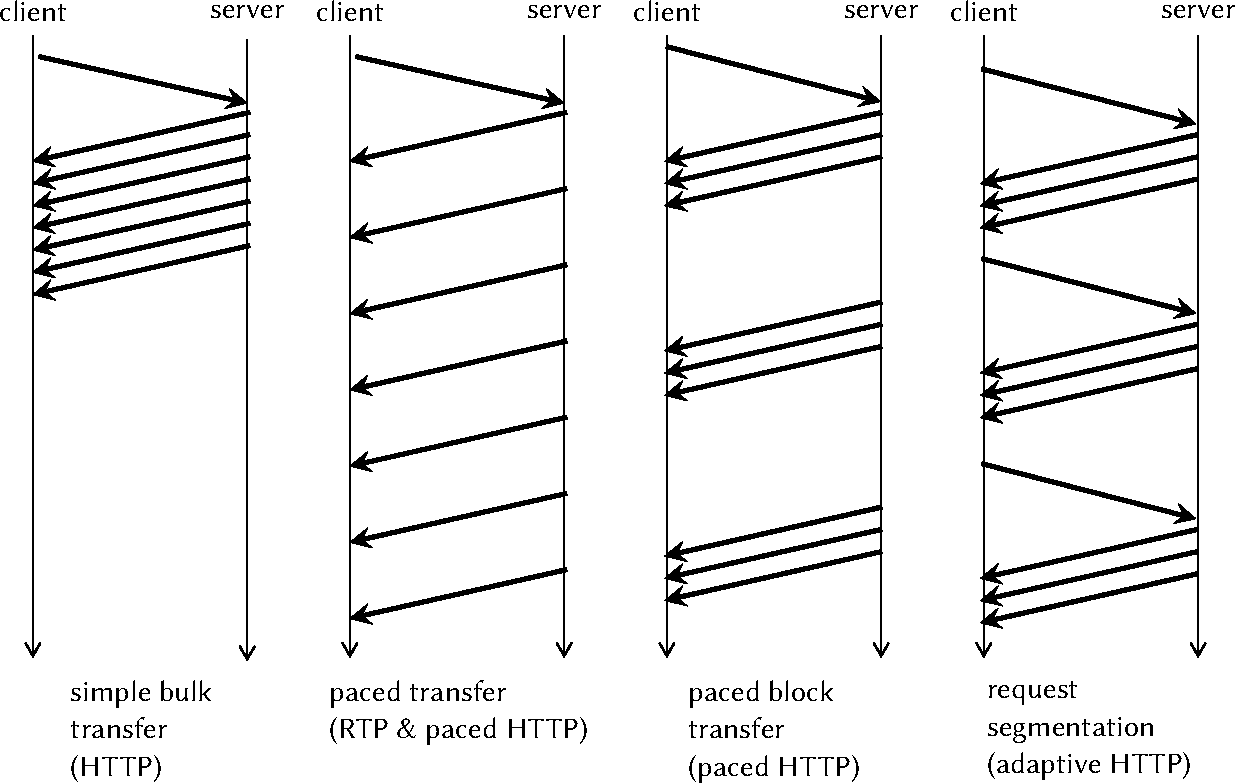
\includegraphics[width=1.0\textwidth]{images/streaming-transfer-modes.pdf}
\caption{Comparison of several possible streaming transfer modes (Source: \cite{ma2011mobile}).}
\label{c3:fig:streamingtransfermodes}
\end{figure}

\item \textit{Video quality and rate adaptation}. To be able to support varying video bitrate levels similar to RTP some adaptations to HTTP streaming are needed. At first, the video has to be encoded multiple times to several output bitrates. Also, the video container needs to be able to support switching the stream at will with everything required for the playback in place. Additionally, an independently available index file needs to correlate the video files with their contents. Alternatively, the video can be segmented into short pieces of several seconds outlined by a separate index file. Then the client can choose the stream variant that best fits its current condition, which depends on parameters including the display size or varying network QoS. \cite{ma2011mobile} gives an overview over some possibilities. Several proprietary protocols, some of them in the process of standardization, tackle this, including HTTP Live Streaming \cite{pantos2011livestreaming} and Microsoft Smooth Streaming \cite{zambelli_iis_2009}. They are either based on file segmentation or HTTP RANGE requests. Initial experiments in \cite{akhshabi2011experimental} evaluate the viability of this kind of approach. We plan to extend this by modelling the fundamental building blocks the mechanisms have in common and after that giving tools to find and evaluate combinations best suited to specific network conditions.
This includes evaluations of the optimal length of segments as well as tuning the aforementioned buffering models to be able to cope with at least two new degrees of freedom, i.e. being able to load multiple segments at once using more than one connection as well as the ability to switch to another video encoding level in case of changing connection capacity or buffer pressure conditions.

\end{itemize}

The focus of the thesis will be to explore the possibility space of the aforementioned mechanisms and give the ability to make informed choices on the viability of them or whole protocols for specific use cases.





%%%%%%%%%%%%%%%%%%%%%%%%%%%%%%%%%%%%%%%%%%%%%%%%%%%%%%%%%%%%%%%%%%%%%%%%%%%%%%%%
\section{Streaming Modeling}




%%%%%%%%%%%%%%%%%%%%%%%%%%%%%%%%%%%%%%%%%%%%%%%%%%%%%%%%%%%%%%%%%%%%%%%%%%%%%%%%
\section{Streaming Quality Determination and Metrics}



%%%%%%%%%%%%%%%%%%%%%%%%%%%%%%%%%%%%%%%%%%%%%%%%%%%%%%%%%%%%%%%%%%%%%%%%%%%%%%%%
\section{FITCE2011 YouTube Streaming Emu INSERT}

%%%%%%%%%%%%%%%%%%%%%%%%%%%%%%%%%%%%%%%%%%%%%%%%%%%%%%%%%%%%%%%%%%%%%%%%%%%%%%%%
\section{Introduction}
\label{sec:introduction}

Web-based video delivery uses the Web's general purpose transfer protocols, primarily HTTP and the underlying TCP transport protocol. The only requirement to participate in this form  of video streaming is either a recent version of one's favorite web browser supporting the HTML5 \texttt{<video>} tag or, becoming less important, a player for Flash content. This user-friendliness opened the curtains for a much broader audience when compared to RTP streaming approaches. Popular examples include sites with user generated content like YouTube which has an especially large number of viewers and high watch duration \cite{comscore2011ranking}, and commercial sites such as Netflix and Hulu. Netflix accounts for 30\% of today's peak downstream Internet traffic in North America \cite{sandvine_spring2011}, also demonstrating the huge demand for this type of service.

The proportion of total Internet traffic shifted hugely towards video transfers in recent years. Google, who operates YouTube since 2006, now carries a large percentage of that traffic \cite{nw2010carrier}. But the Internet's traffic volume is expected to continue to rise in the next years. If the underlying network infrastructure is not upgraded at the the same speed, this could result in performance degradations for the Internet. Moreover, mobile networks struggle with limited and shared bandwidths, high delay and considerable loss due to intrinsic radio problems, even with new and upcoming mobile specifications such as LTE. Web-based video delivery does not use specialized streaming techniques such as quality scaling, loss tolerance or dedicated signaling connections, but still needs to be able to work well even under theses circumstances



This paper investigates how Web-based media delivery works in general, and how meaningful measurement of its streaming quality can be achieved with future network developments and degraded network parameters in mind.

As YouTube is one of the largest world-wide operating Web streaming contenders it is the focus of our attention in this paper. After giving a brief overview of the tackled research areas in Section \ref{chap:relatedwork} we make initial insights into YouTube's network architecture in Section \ref{sec:videodeliveryarchitecture} and cover the basics of HTTP streaming in Section \ref{sec:featureshttpstreaming}. we move on to describe the underlying models used in the streaming process and the metrics we intend to use in the observations in Section \ref{sec:metricsmodel}. Finally, Section \ref{sec:measurements} covers the video streaming measurements, and Sections \ref{sec:outlook} and \ref{sec:conclusion} give and outlook and conclude the paper.






%%%%%%%%%%%%%%%%%%%%%%%%%%%%%%%%%%%%%%%%%%%%%%%%%%%%%%%%%%%%%%%%%%%%%%%%%%%%%%%%
\section{Video Delivery Architecture}
\label{sec:videodeliveryarchitecture}


Large Internet sites are not hosted at one central site anymore, but are usually served through geographically distributed entities forming a load-balancing structure. Such load balancing mechanisms have a long history on the Web, e.g. in the form of mirror servers a user can select manually.

In today's Content Distribution Networks (CDN), a much larger number of mirror servers is available, and selection of a server is no longer carried out explicitly by the user, but implicitly through DNS: Content is addressed using URLs (\texttt{http://somedomain/somepath} in its simplest form), and the CDN's DNS servers are configured to resolve certain domain names to different IP addresses, depending on where the query originated.

To get an insight into the structure of YouTube's content distribution network, we undertook a two-step measurement campaign \cite{rafetseder2011explyt}. First, we downloaded and manually parsed the HTML code served by YouTube's web servers. We could thus enumerate and learn about the structure of domain names in the system. The most relevant category of domain names for our purposes takes the form of \texttt{v$\alpha$.lscache$\beta$.c.youtube.com}, where $0<\alpha<25$ and $0<\beta<9$. Not all permutations of names are found at all times. We also noted that there are hostnames that seem to point to geographical locations, but have not succeeded so far in exhaustively mapping those two types of names.

The second part of our campaign consisted of active measurements on forty distributed computers (part of the \textit{Seattle} Internet testbed\footnote{\url{https://seattle.poly.edu/html/}} \cite{Cappos:2009:SPE:1508865.1508905}) for over 600 hours. We learned that the frontend web server name, \texttt{www.youtube.com}, resolves to multiple IP addresses per geographical location of the probing host which are mostly disjoint from sets of addresses found on other hosts. The number of frontend IP addresses also changes over time, e.g. to account for load variations such as load increases during the evening hours in the hosts' time zones. The actual video cache servers only have one IP address per name and location each, but sometime this address is seen to change during the day. 

When looking at the resolved addresses per frontend server and time zone, two interesting time-dependent scaling effects can be seen: First, servers become reachable or vanish in a coordinated manner controlled by the time of day, i.e. in a 24 hour pattern. We speculate this provides a gain in efficiency for the overall system to turn on parts of the resource pool for load balancing only when there is demand.

The second type of effect occurs much more seldom. It stretches out over multiple days and is best described as follows: A new block of server IP addresses is made available in addition to the existing ones. After a few days of parallel operation, a previously active block is taken out of service. The new block continues to serve. Comparison measurements  performed in parallel show that this switch-over between IP address blocks has a positive effect on the latency to the servers, as the latency to non-YouTube destinations show no improvements at all.





%%%%%%%%%%%%%%%%%%%%%%%%%%%%%%%%%%%%%%%%%%%%%%%%%%%%%%%%%%%%%%%%%%%%%%%%%%%%%%%%
\section{Features of HTTP Streaming}
\label{sec:featureshttpstreaming}

The leitmotif of HTTP streaming is the inversion of control compared to RTP streaming. Due to UDP's lack of reliability, congestion control, and flow control features, RTP does need to do this on its own. Therefore, the RTP server application is responsible to implement and conduct these, increasing its complexity. Even playback control is done by the server, albeit at the request of the client. Web-streaming turns this around and puts the client in charge. Because HTTP streaming relies on TCP explicit server control is unnecessary. Control is now done either implicitly by the transport protocol or explicitly by the client, e.g. playback control which also plays an important role in buffer management. This inversion also eliminates the need to exchange client metrics to the server, but increases the complexity of the client. Moreover, TCP's reliable transport feature may prove to negatively affect playback in suboptimal network conditions.

%Because HTTP streaming relies on TCP this is not necessary, but it also removes a bit of flexibility, as the type of congestion control is given. 


In its simplest form Web streaming acts like regular HTTP traffic. The video is requested and then delivered from the server in one single block transfer. The transfer is controlled by the server and it can employ pacing mechanisms to somewhat match the download duration to the playback duration. This reduces load spikes and the required buffer size on the client device but also makes the process more vulnerable to changing network conditions. YouTube uses a server-side pacing mechanism which is  discovered in \cite{alcock2011afcyt}\footnote{\url{http://www.wand.net.nz/~salcock/youtube/}} and also discussed in Section \ref{sec:measurements}.

These simple mechanisms, however, can not seamlessly change quality in a currently running video. This can be important for, e.g., mobile networks or when an increasingly loaded server can not fulfill every request in its highest quality at the required speed anymore.

Therefore adaptive forms of HTTP streaming were developed. The techniques complement and extend the server-side pacing mechanisms and introduce video quality and bitrate adaption to HTTP streaming by doing file segmentation \cite{ma2011mobile, watching-video1}. Bitrate adaption, belonging to a class of application-layer flow control mechanisms, can add an extra level of feedback to react to changing network conditions but could also make buffer management more complex. Protocols based on this approach are already widespread, e.g. in Netflix's offerings.





%%%%%%%%%%%%%%%%%%%%%%%%%%%%%%%%%%%%%%%%%%%%%%%%%%%%%%%%%%%%%%%%%%%%%%%%%%%%%%%%
\section{Metrics and Model}
\label{sec:metricsmodel}

\begin{figure}[htbp]
%\vskip -2.5cm
        \centering
        % \begin{subfigure}[b]{0.50\textwidth}
        %         \centering
        %         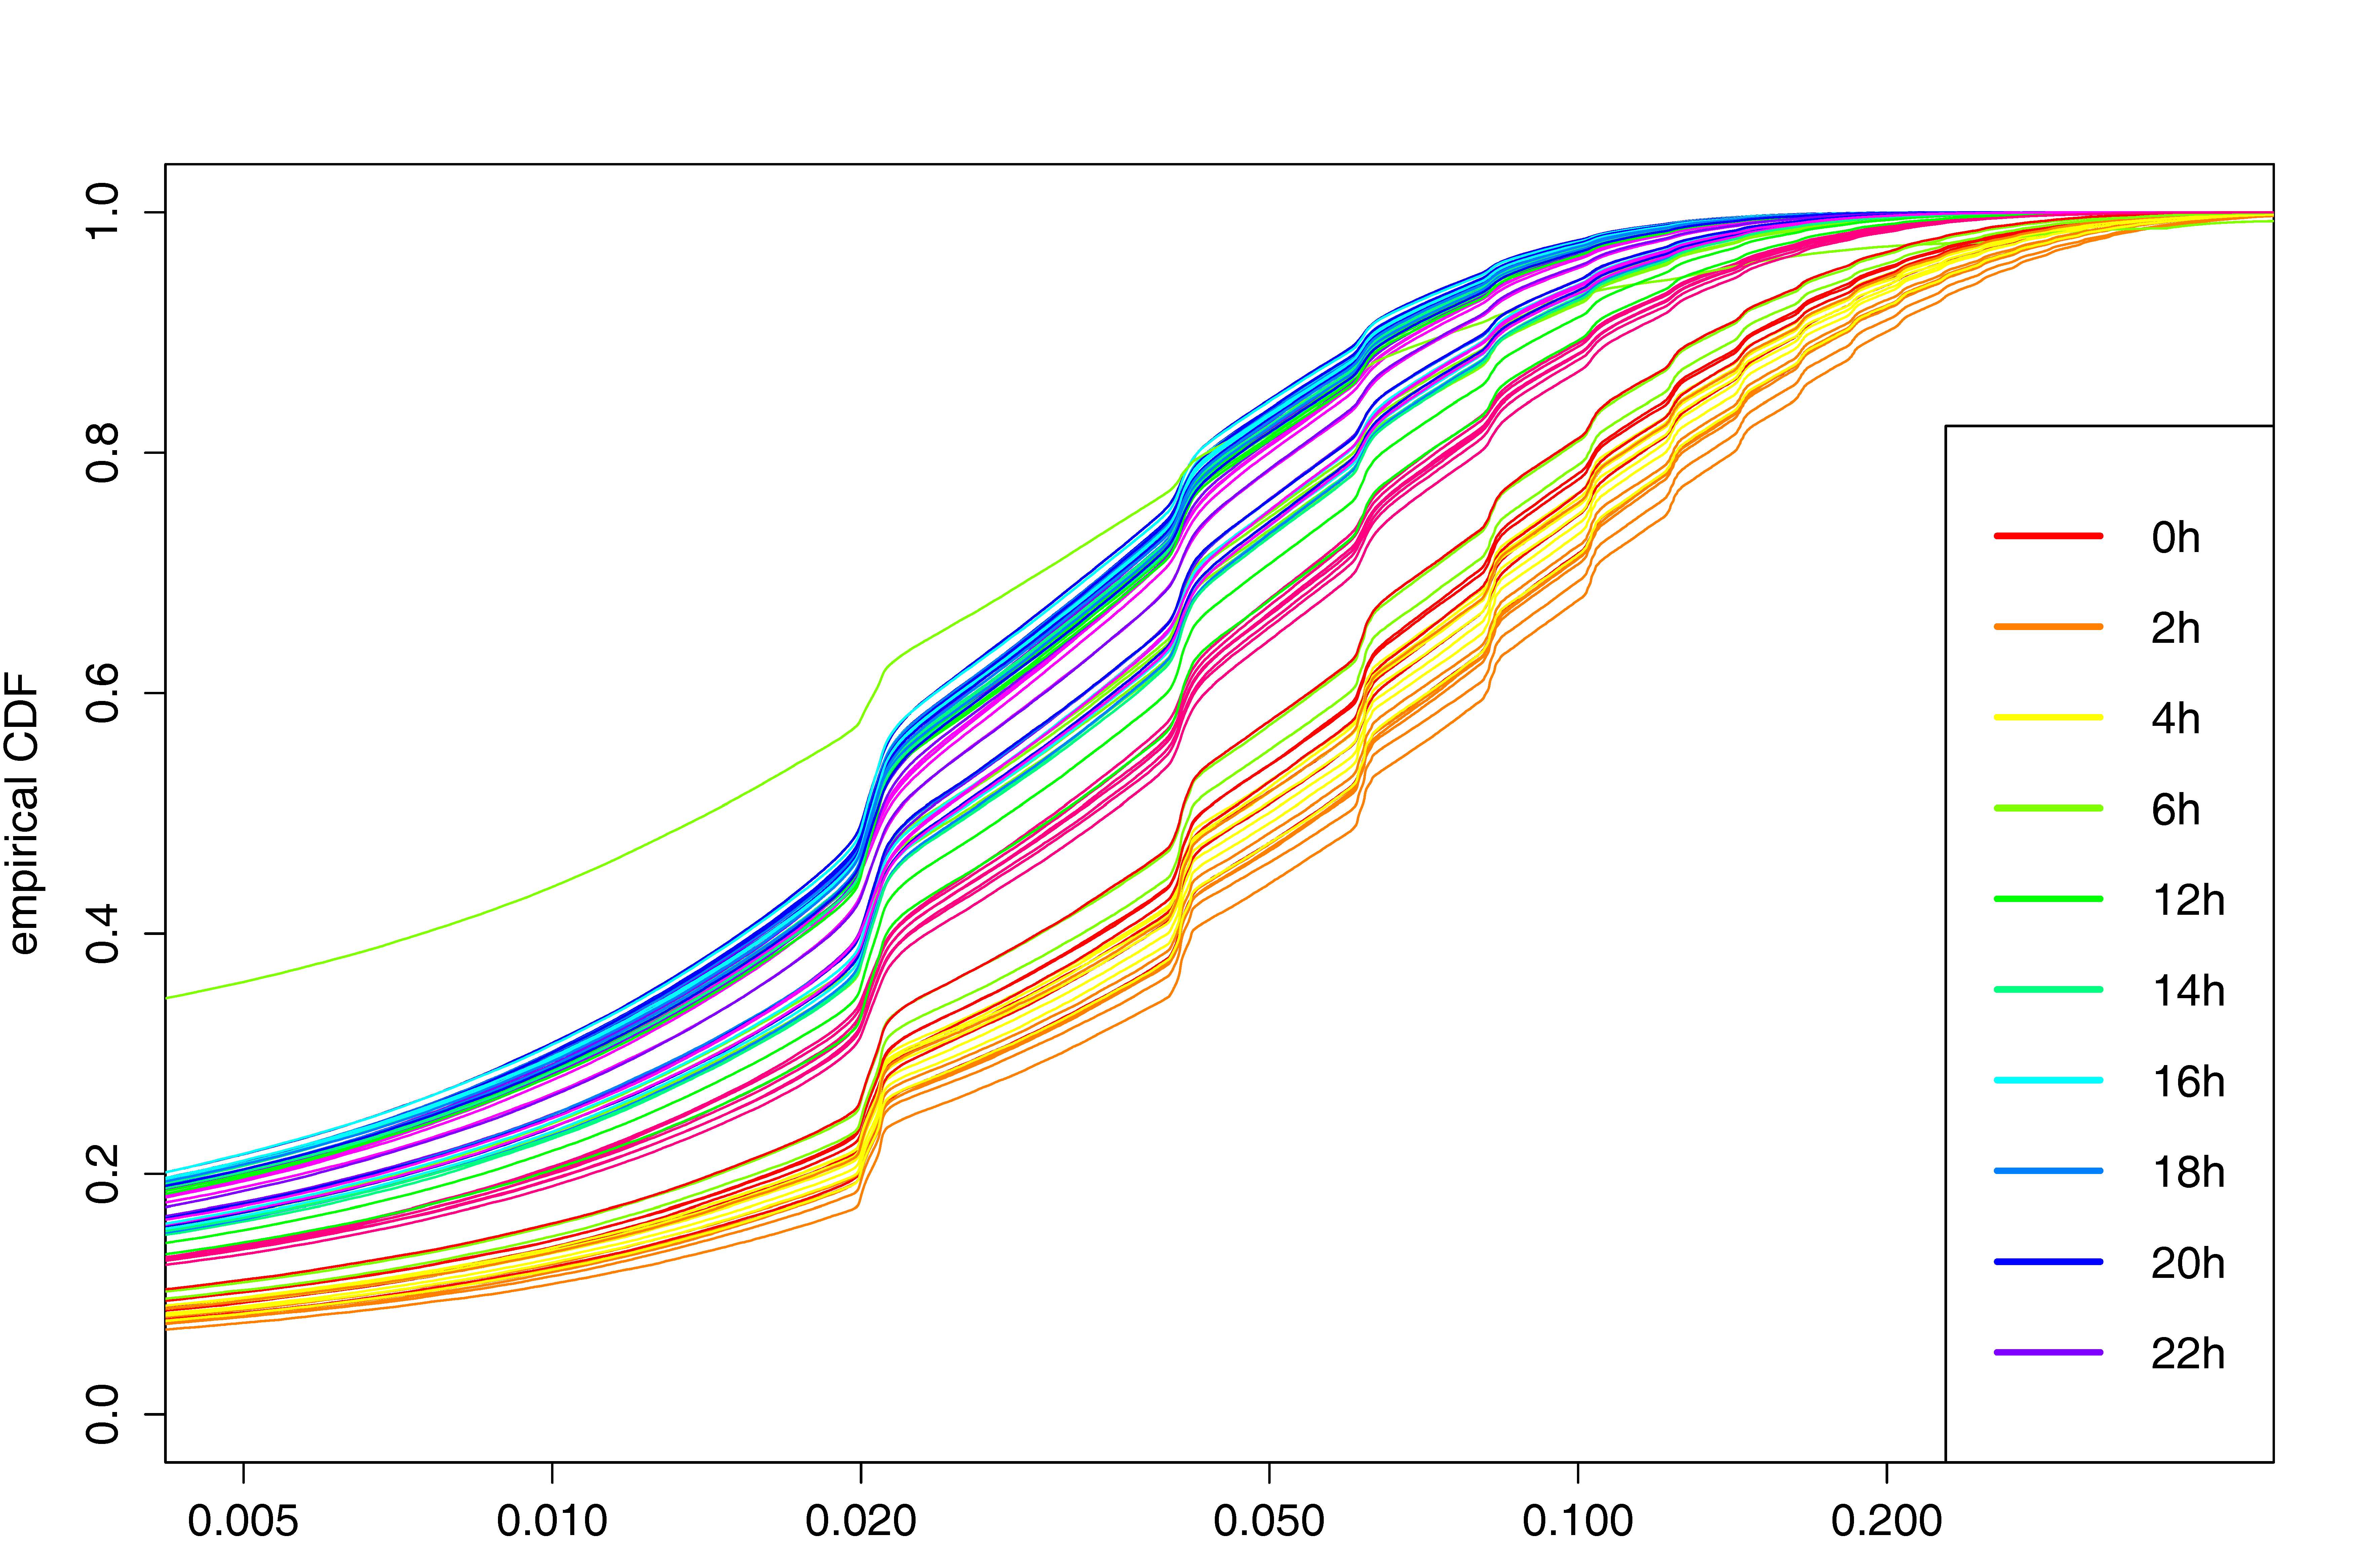
\includegraphics[width=\textwidth]{figures/R-IAT-ecdf-2h-log.png}
        %         \caption{All incoming tunnel requests.}
        %         \label{fig:IAT-ecdf-2h-all}
        % \end{subfigure}%
        %~ %add desired spacing between images, e. g. ~, \quad, \qquad etc.
          %(or a blank line to force the subfigure onto a new line)
        \begin{subfigure}[b]{0.50\textwidth}
                \centering
                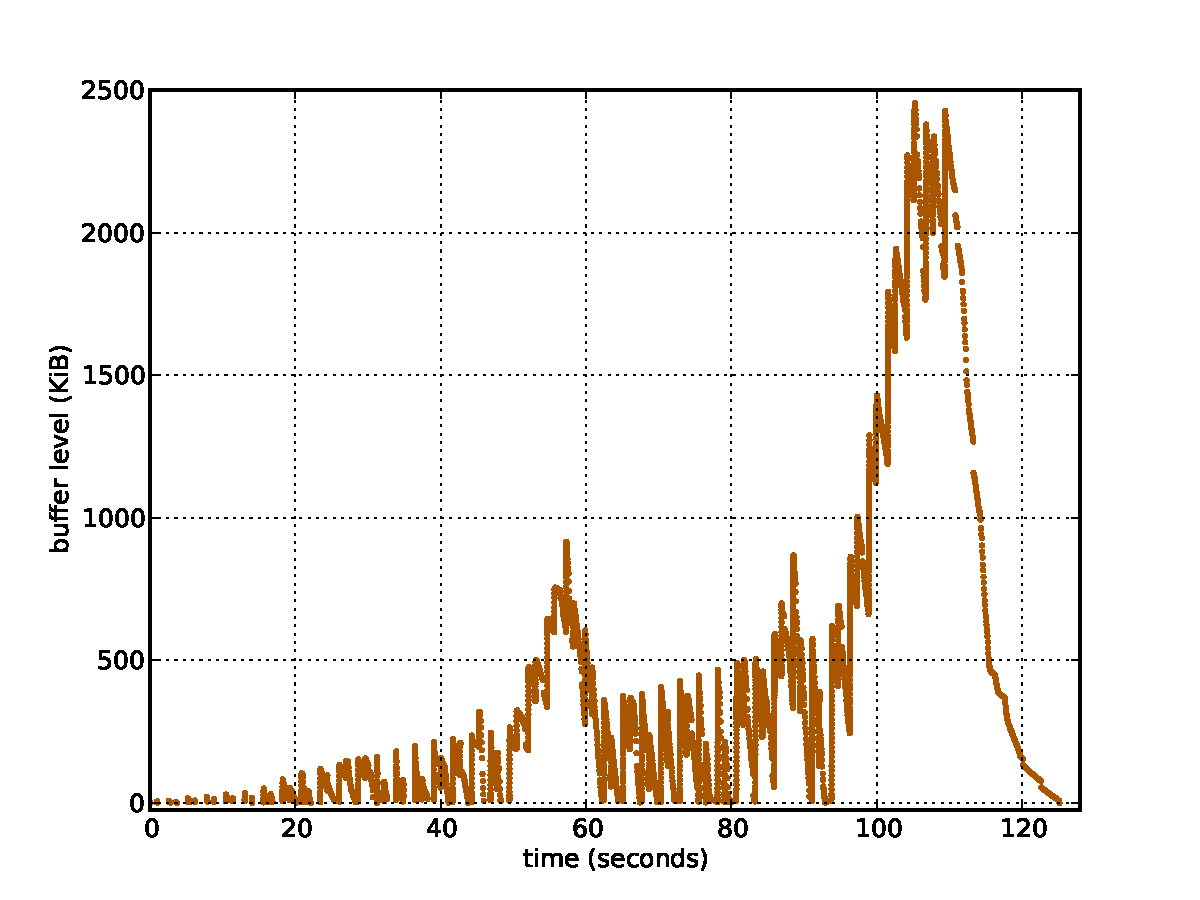
\includegraphics[width=\textwidth]{images/bufferlevel-stall-new.pdf}
                \caption{Playback stalling method, 33s total stalling.}
                \label{c3:fig:bufferlevel-stall}
        \end{subfigure}%
        ~
        \begin{subfigure}[b]{0.50\textwidth}
                \centering
                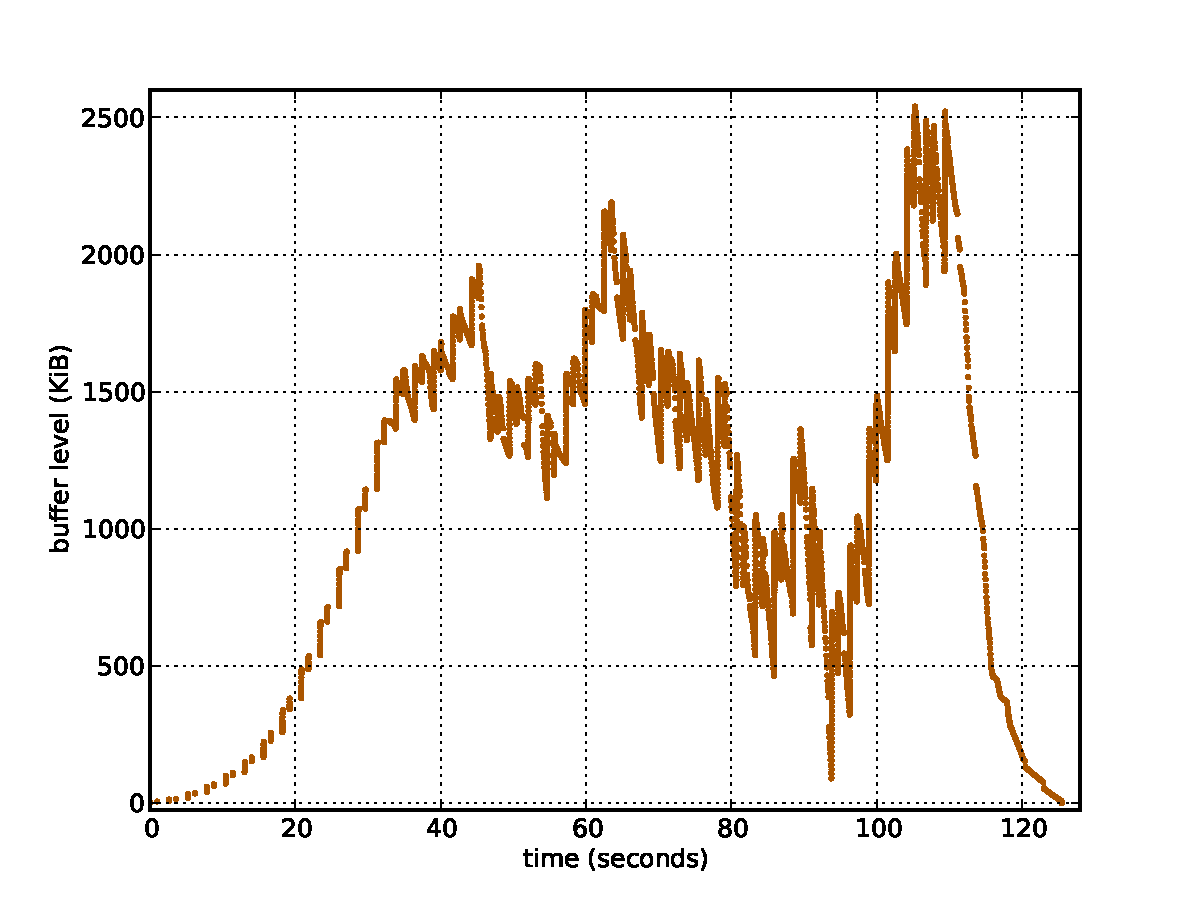
\includegraphics[width=\textwidth]{images/bufferlevel-startdelay-new.pdf}
                \caption{Delayed playback method, 33s total stalling.}
                \label{c3:fig:bufferlevel-startdelay}
        \end{subfigure}

        \begin{subfigure}[b]{0.50\textwidth}
                \centering
                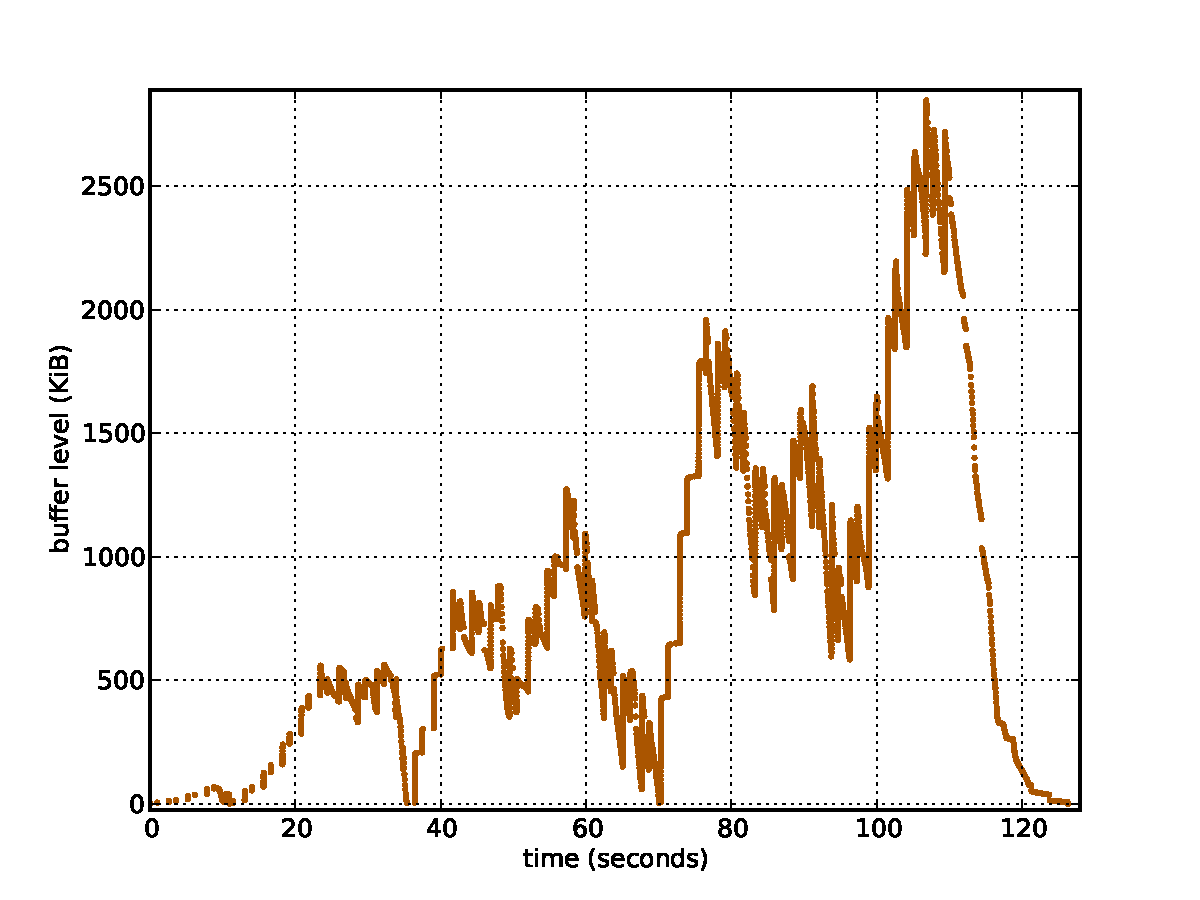
\includegraphics[width=\textwidth]{images/bufferlevel-flash-new.pdf}
                \caption{YouTube Flash Player method, 34s total stalling.}
                \label{c3:fig:bufferlevel-flash}
        \end{subfigure}%
        ~
        \begin{subfigure}[b]{0.50\textwidth}
                \centering
                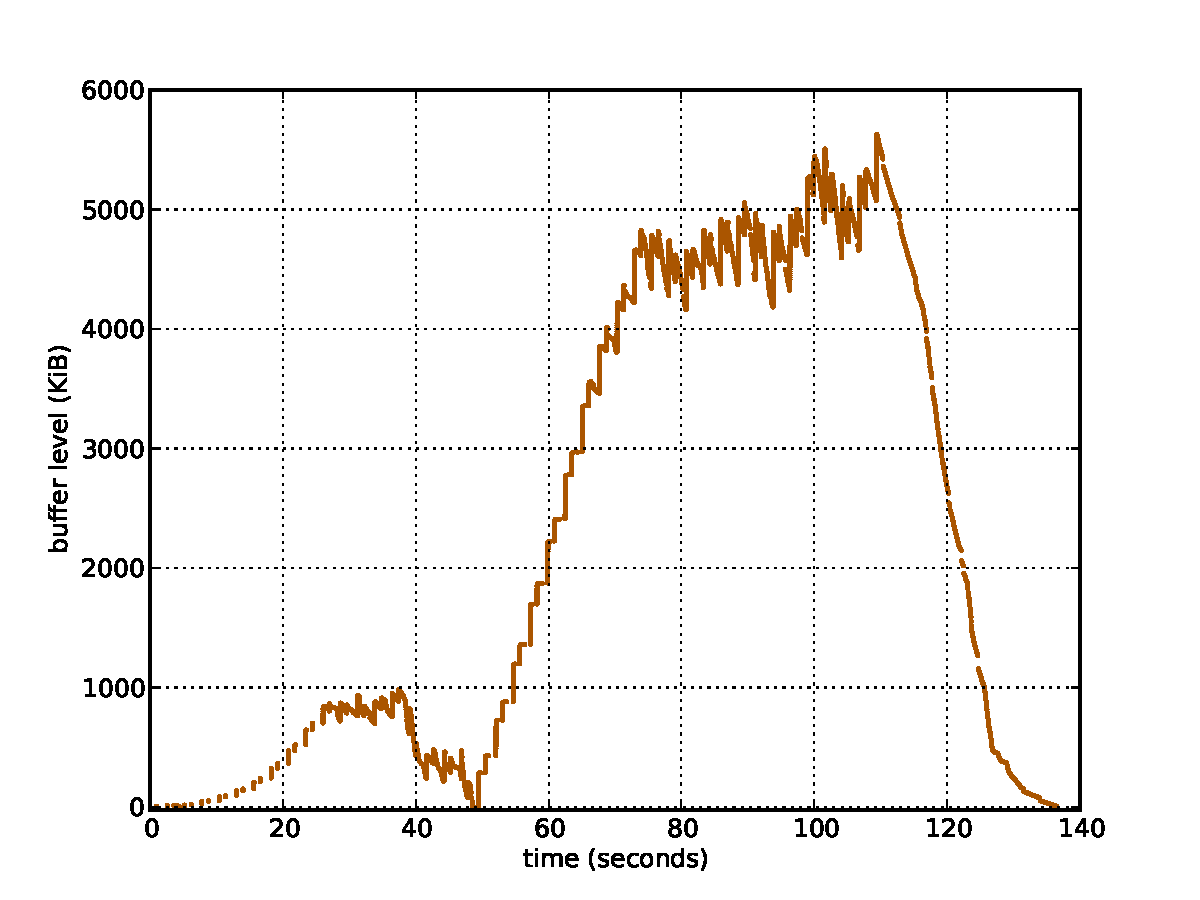
\includegraphics[width=\textwidth]{images/bufferlevel-firefox-new.pdf}
                \caption{Firefox 4 method, 44s total stalling.}
                \label{c3:fig:bufferlevel-firefox}
        \end{subfigure}
\caption{Modelled buffer fill level graphs and resulting total stalling times.}
\label{c3:fig:bufferlevel-PV}
\end{figure}
% used yt-delay/hPUGNCIozp0_delay_2500 1, spyder, color #aa5500
% data
% start delay 33s 
% flash 33.82s
% stalling 32.68s
% html5 as implemented in firefox 44s

As web-based delivery uses reliable TCP transfers and (in its simplest form) does not use any kind of scaling or multi-layered video encoding, there will never be any change in the actual video quality. Therefore, the users' experience is influenced by only a small number of parameters. A user will notice some delay after he starts the video streaming process. If the video download is slower than the average video bitrate the playback will stall, i.e. stop playing, at some point until there is enough data available to resume playing again.
The QoS parameters affecting these metrics are limited bandwidth, packet loss, and latency, causing the player to intermittently pause playback and enter a re-buffering state.

Directly measuring these two factors in a user-controlled browser does have drawbacks. The need for user interaction would hamper the effort of creating fully automated measurement series and getting reproducible results. Interfacing with the closed-source Flash software and getting meaningful results can also be a large hurdle.

To achieve increased flexibility we created several models that emulate the streaming process and its buffering and playback behavior. These are based on typical user playback solutions, e.g. a Web browser with a Flash plug-in. For this comparison we used a video of about 90 seconds length and network conditions that could not fulfill the video bitrate in time and hereby forced stalling to occur.

While these models try to give dimensions and characteristics to the initial start delay and the frequency and lengths of stalls they do not directly answer the question of user satisfaction. Approaches to correlate the  measurable parameters and the user satisfaction are tackled in, e.g., \cite{ketyko2010qoe, mokmeasuring, gustafsson2008measmmmquality} and will also be a topic of our future work.



\subsection{Simple Stalling Model}

The simplest version of the model is represented in Figure \ref{c3:fig:bufferlevel-stall} which shows the difference between the aggregate downloaded and already played data, which is the buffer level. The model starts and advances playback immediately when it has enough data to show a full frame and stops every time the buffer is about to run out and restarts immediately when there is data to show. This results in numerous stops and a large loss in playback continuity. However, this model also has the shortest total stalling time and can therefore act as a reference baseline to compare the performance of the other models against it.


\subsection{Simple Predictive Model}

The second approach in Fig. \ref{c3:fig:bufferlevel-startdelay} defers the playback start as long as it is needed to play the video uninterrupted, meaning that the playback buffer will never run out of data. However, this approach is only viable with a complete knowledge over the downloading process, which can only be estimated in live scenarios. Because playback is done with global knowledge and at the earliest point possible the total stalling time is also 33 seconds, but only one long stalling phase occurs while the user initially waits for the playback to start.


\subsection{YouTube Model}

This model tries to resemble the playback mechanisms as implemented in YouTube's Flash video player.
It defers the start until at least two seconds of video data are buffered. When a stall occurs the player buffers at least five seconds of video before restarting. The model does not use any knowledge about the transmission (e.g. current bandwidth).
The result can be seen in Figure \ref{c3:fig:bufferlevel-flash}. Compared to the simple stalling model it increases the playback stability while only marginally affecting the total stalling time, resulting in 34 seconds of stalling.

\subsection{HTML5 Predictive Model}
The standard playback and buffering process of HTML5 is described in the HTML5 specification but adds up to:
\textit{``[...] the user agent [...] will automatically begin playback of the media resource as soon as it can do so without stopping.''} \cite{html5video}. The model presented here is based on the HTML5 implementation of the open source Firefox Browser in version 4 which differs slightly from the HTML standard. Because it is an online algorithm which does not have global knowledge of the video and transmission speeds of any point in the future it has to estimate these. It does so by calculating the moving averages of both. Playback is started when one of these conditions are met:

\begin{itemize}
\item The player has been buffering data for at least 30 seconds.
\item The player has already buffered an amount of data corresponding to 30 seconds of video.
\item The video download has been completed.
\item The moving average of the transmission rate is larger than the moving average of the video bitrate and the player has a safety buffer with 20 seconds of video data.
\end{itemize}

This approach is quite conservative and trades longer waiting times for fewer interruptions. The test case for our model is shown in Figure \ref{c3:fig:bufferlevel-firefox}. Initially, playback starts only after a long waiting period of about 25 seconds. Also, the only intermittent stall causes a long buffering period. Then again, the model keeps the total number of stalls down to this single stall. However, due to the longer overall stalling time of 44 seconds the player needs to buffer more data than the other model implementations. In our test case the maximum buffer size increased from about 2800 KiB to 5600 KiB. This may be a problem for devices with sparse amounts of memory, e.g. mobile telephones or small dedicated streaming boxes. However, a large buffer can also increase the chance of continuous playback in mobile scenarios with intermittent service interruption.


%Which offers better quality to users? Some approaches (TODO: refs and explain how)

% Longer waiting time but very few stops. Stalling model definitely the shortest waiting time but stops too frequent with insufficient network conditions, i.e. can not really be used. Delayed playback requires total knowledge not available beforehand. Can maybe used with reduced information, bandwidth estimation, but this is essentially HTML5/Firefox.




%%%%%%%%%%%%%%%%%%%%%%%%%%%%%%%%%%%%%%%%%%%%%%%%%%%%%%%%%%%%%%%%%%%%%%%%%%%%%%%%
\section{Measurements}
\label{sec:measurements}

%TODO:
%comment on which buffering model is used, both simple models result in smallest buffering time possible, as no overhead waiting is involved

For the YouTube streaming measurements we implemented an automated video downloading and playback simulation software to feed information into the model and evaluate the total stalling time. For this the simple stalling model is used because this results in the shortest possible playback duration in every scenario. Furthermore, we used a network emulation testbed to subject the video streaming to increased loss and latency while fixing the maximum network bandwidth and observe the influence on the QoE.

The first point of interest discovered during the evaluation of the measurements was the information encoded in the URLs pointing to the actual video files (cf. Table \ref{c3:tbl:yturl}) as they hinted on the presence of transmission rate throttling for some videos. However, if one tries to alter or remove the throttling parameters the YouTube server responds to this with a HTTP 403 forbidden error code, meaning that there are further checks in place to ensure this behavior. 

We experienced this hinted throttling for all non-HD (i.e. lower than 720p resolution) videos. The throttling method, which \cite{alcock2011afcyt} also observed, limits the transmission to a rate higher than but correlated to the average media bitrate. The \textit{block-sending} method used for the limiting is rather unusual as it transmits short packet bursts, typically 64 KiB in size, followed by long pauses as seen in Figure \ref{c3:fig:blocktransfer-detail}. Initially, a larger burst is transmitted to allow for some pre-buffering to occur in the client's media player (cf. Fig. \ref{c3:fig:blocktransfer-overall}). This limiting is probably in place to even the load on the caches and to prevent load spikes, yet ensuring that every client receives the necessary data in time for playback.



\begin{figure}[htbp]
% used yt-delay/hPUGNCIozp0_delay_100 2, spyder with matplotlib config patch
	\centering
    	\begin{subfigure}[b]{0.80\textwidth}
                \centering
                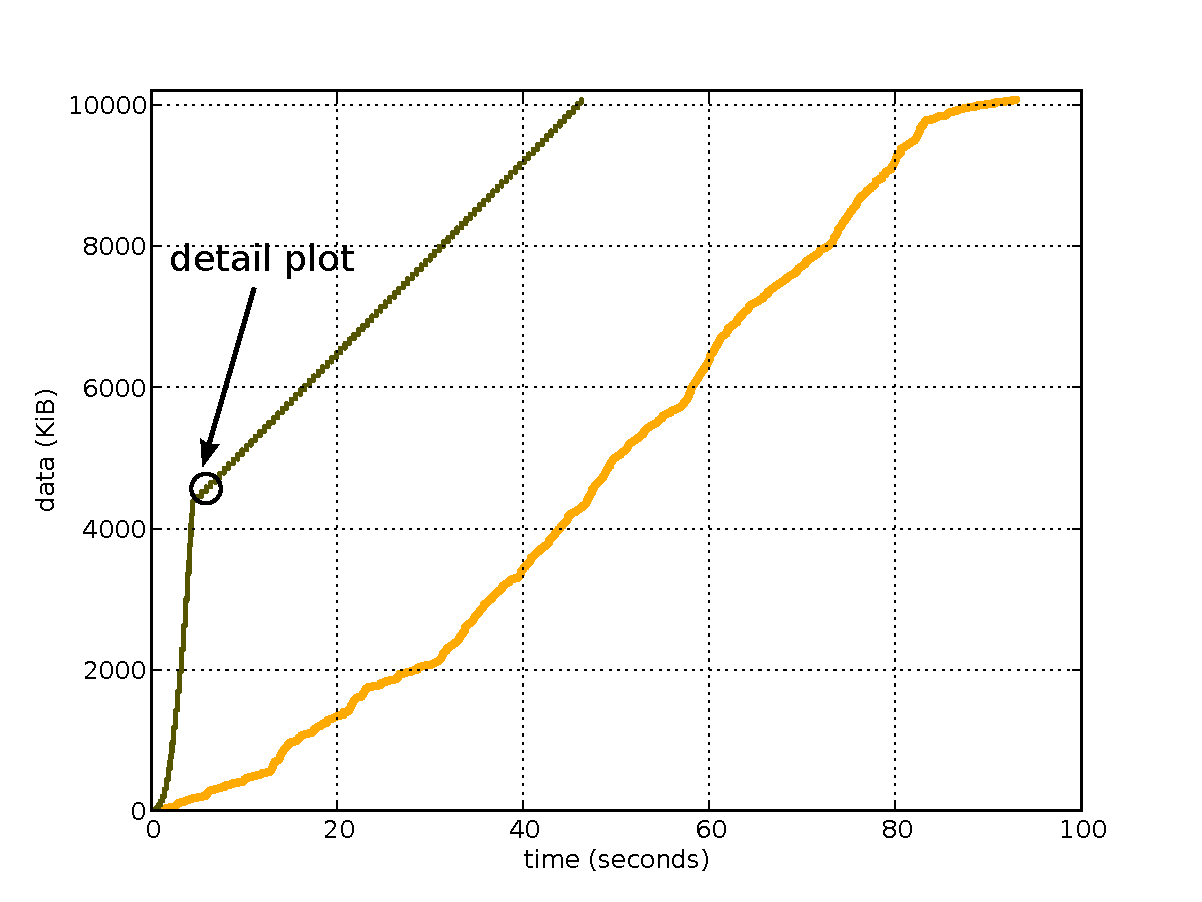
\includegraphics[width=\textwidth]{images/blocktransfer-mod.pdf}
                \caption{Overall graph.}
                \label{c3:fig:blocktransfer-overall}
        \end{subfigure}

    	\begin{subfigure}[b]{0.80\textwidth}
                \centering
                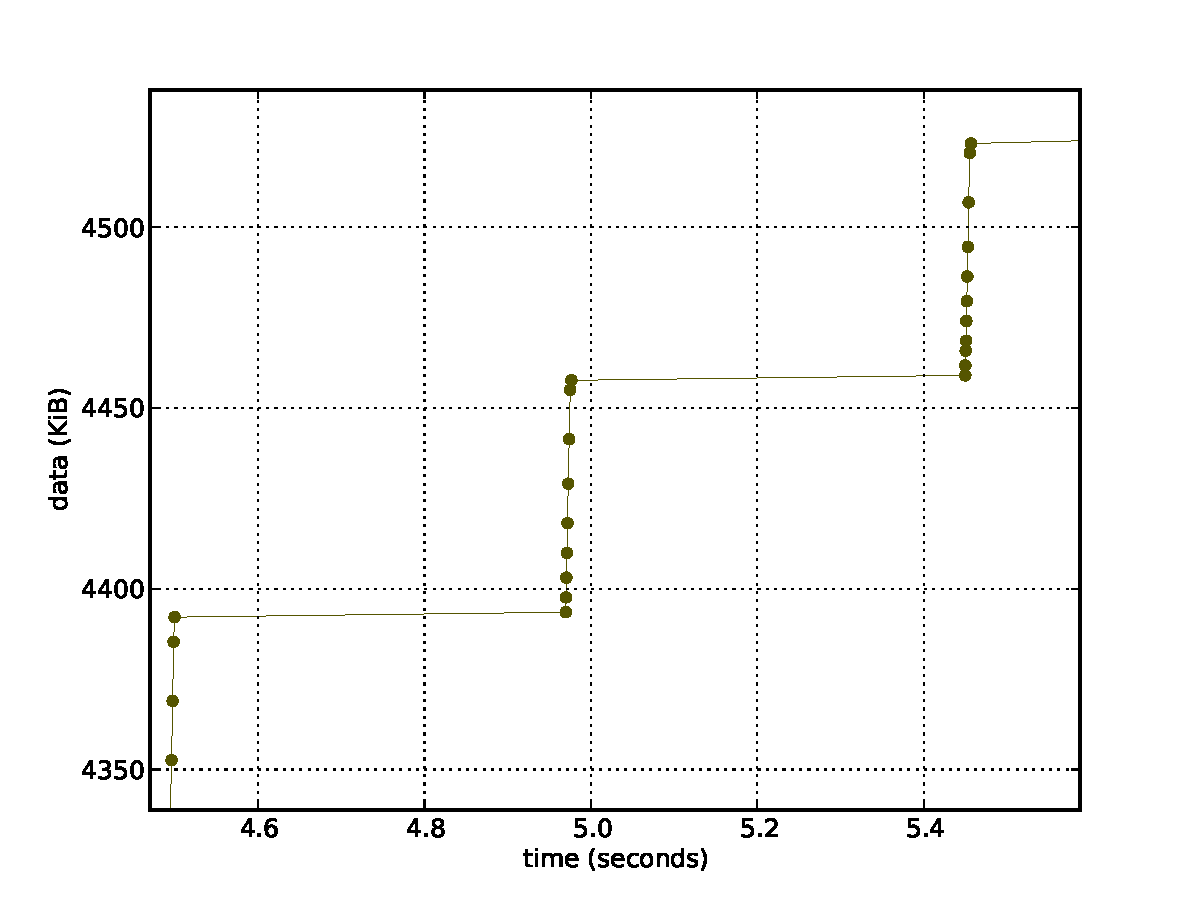
\includegraphics[width=\textwidth]{images/blocktransferdetail.pdf}
                \caption{Detail plot of the rate-limited block-sending phase.}
                \label{c3:fig:blocktransfer-detail}
        \end{subfigure}
\caption{Measurement results for the download and playback of a video.}
\label{c3:fig:blocktransfer}
\end{figure}



\begin{table}[htbp]
% increase table row spacing, adjust to taste
\renewcommand{\arraystretch}{1.3}
\caption{Transmission Related Parameters from YouTube's Video URL Setup}
\label{c3:tbl:yturl}
\centering
\begin{tabular}{|p{4.7cm}||p{3.3cm}|}\hline
URL Part & Description \\ \hline \hline
\texttt{v$\alpha$.lscache$\beta$.c.youtube.com} &  Cache server involved in the delivery.\\ \hline
%\texttt{expire=<UNIX Epoch>} & Describes temporal validity of the URL.\\ \hline
%\texttt{itag=<DIGIT>} and \texttt{signature=<40xHEX>.<40xHEX>} and \texttt{id=<16xHEX>} & Video identification parameters.\\ \hline
\texttt{algorithm=throttle-factor} and \texttt{burst=40} and \texttt{factor=1.25} & Indicates initial burst plus block sending configuration. \\ \hline
\texttt{ratebypass=yes} & Parameter to indicate no rate limiting.\\ \hline
\end{tabular}

\end{table}

We performed two measurement series, one with increased packet loss, the other one adding latency to the path. For each value of loss and latency a mean total stalling time was calculated out of five separate experiments to eliminate temporal and network load influences. Additionally, standard deviations are shown in the resulting graphs of Figure \ref{c3:fig:seriesgraphs}. We clearly notice very large deviations in some experiments. Some of these can be explained by connection timeouts and later resumption of the streaming. Furthermore, an exponential regression line shows the trend of the total stalling times in the experiments.


Figure \ref{c3:fig:delayseries} displays the results of of the latency measurement series with up to five seconds of additional delay. In the worst case the stalling time increases to about 50 seconds. In mobile scenarios latencies of up to 2 seconds can be expected, which would, according to our measurements, result in a maximum mean stalling time of 15 seconds for a 90 second video, which could very well be bearable for YouTube users.

There are several factors that could contribute to the increase in stalling time in the latency experiments. 
TCP, in its simplest form, increases the congestion window based on the Round Trip Time (RTT), making it highly dependent on this connection parameter. Newer congestion avoidance algorithms, e.g. the CUBIC algorithm used in Linux \cite{ha2008cubic}, however reduce this dependence on the RTT.
Another influencing factor might be YouTube's block sending mechanism, which, according to \cite{alcock2011afcyt}, may negatively interact with congestion control algorithms. The impact of packet loss on stalling is much higher than that of latency in our measurements. Yet, due to TCP's reliable transmissions, loss only causes increased packet retransmissions, and, thus, acts as a source of burst delay which negatively impacts the overall throughput.

Figure \ref{c3:fig:lossseries} shows the series of loss experiments. While the 6\% packet loss and below has an almost negligible influence on the stalling time anything above this value will probably not achieve good user experience at all. Interesting to note is the rather sudden increase in stalling time when there is more than 6\% loss added. This could again hints to the transport protocol's reliable transport feature, which catches all the occurring losses, through timeouts or gaps in the sequence numbers. However, the detection and retransmission takes some time, which is reflected in the increased stalling time.





% TODO: Mobile video delivery with HTTP \cite{ma2011mobile}
% reasoning for "HTTP pacing" and segmented delivery

\begin{figure}[htbp]
% yt-delay-allBW.ods, graphik aus LibreOffice Calc, OLE in LibreOffice Draw, font sizes min 11pt, Page Margins passen (18,2 x 10,3), als PDF exportiert.
% new method: extra libreoffice calc page, scaled to fit on one page, pdf export, cut with acrobat
	\centering
    	\begin{subfigure}[b]{1.0\textwidth}
                \centering
                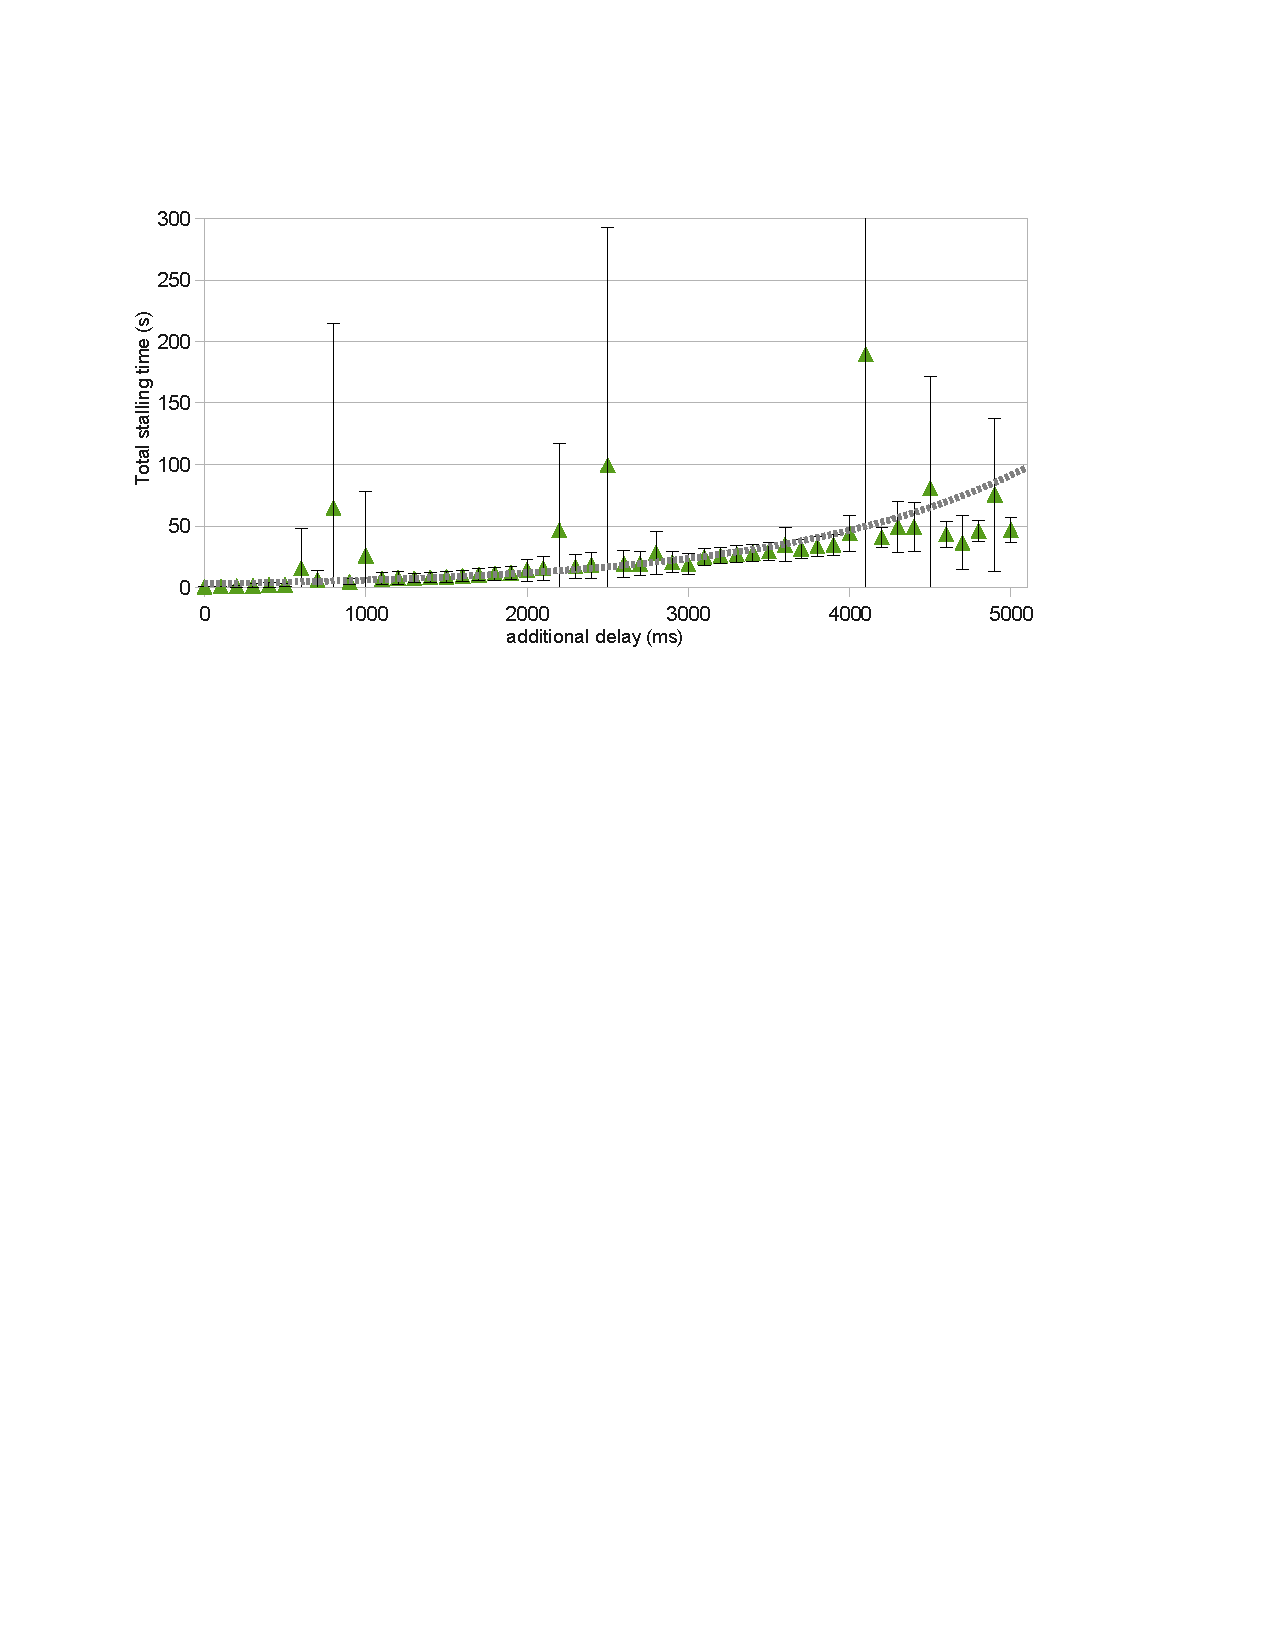
\includegraphics[width=\textwidth]{images/delay.pdf}
                \caption{Latency Graph.}
                \label{c3:fig:delayseries}
        \end{subfigure}

    	\begin{subfigure}[b]{1.00\textwidth}
                \centering
                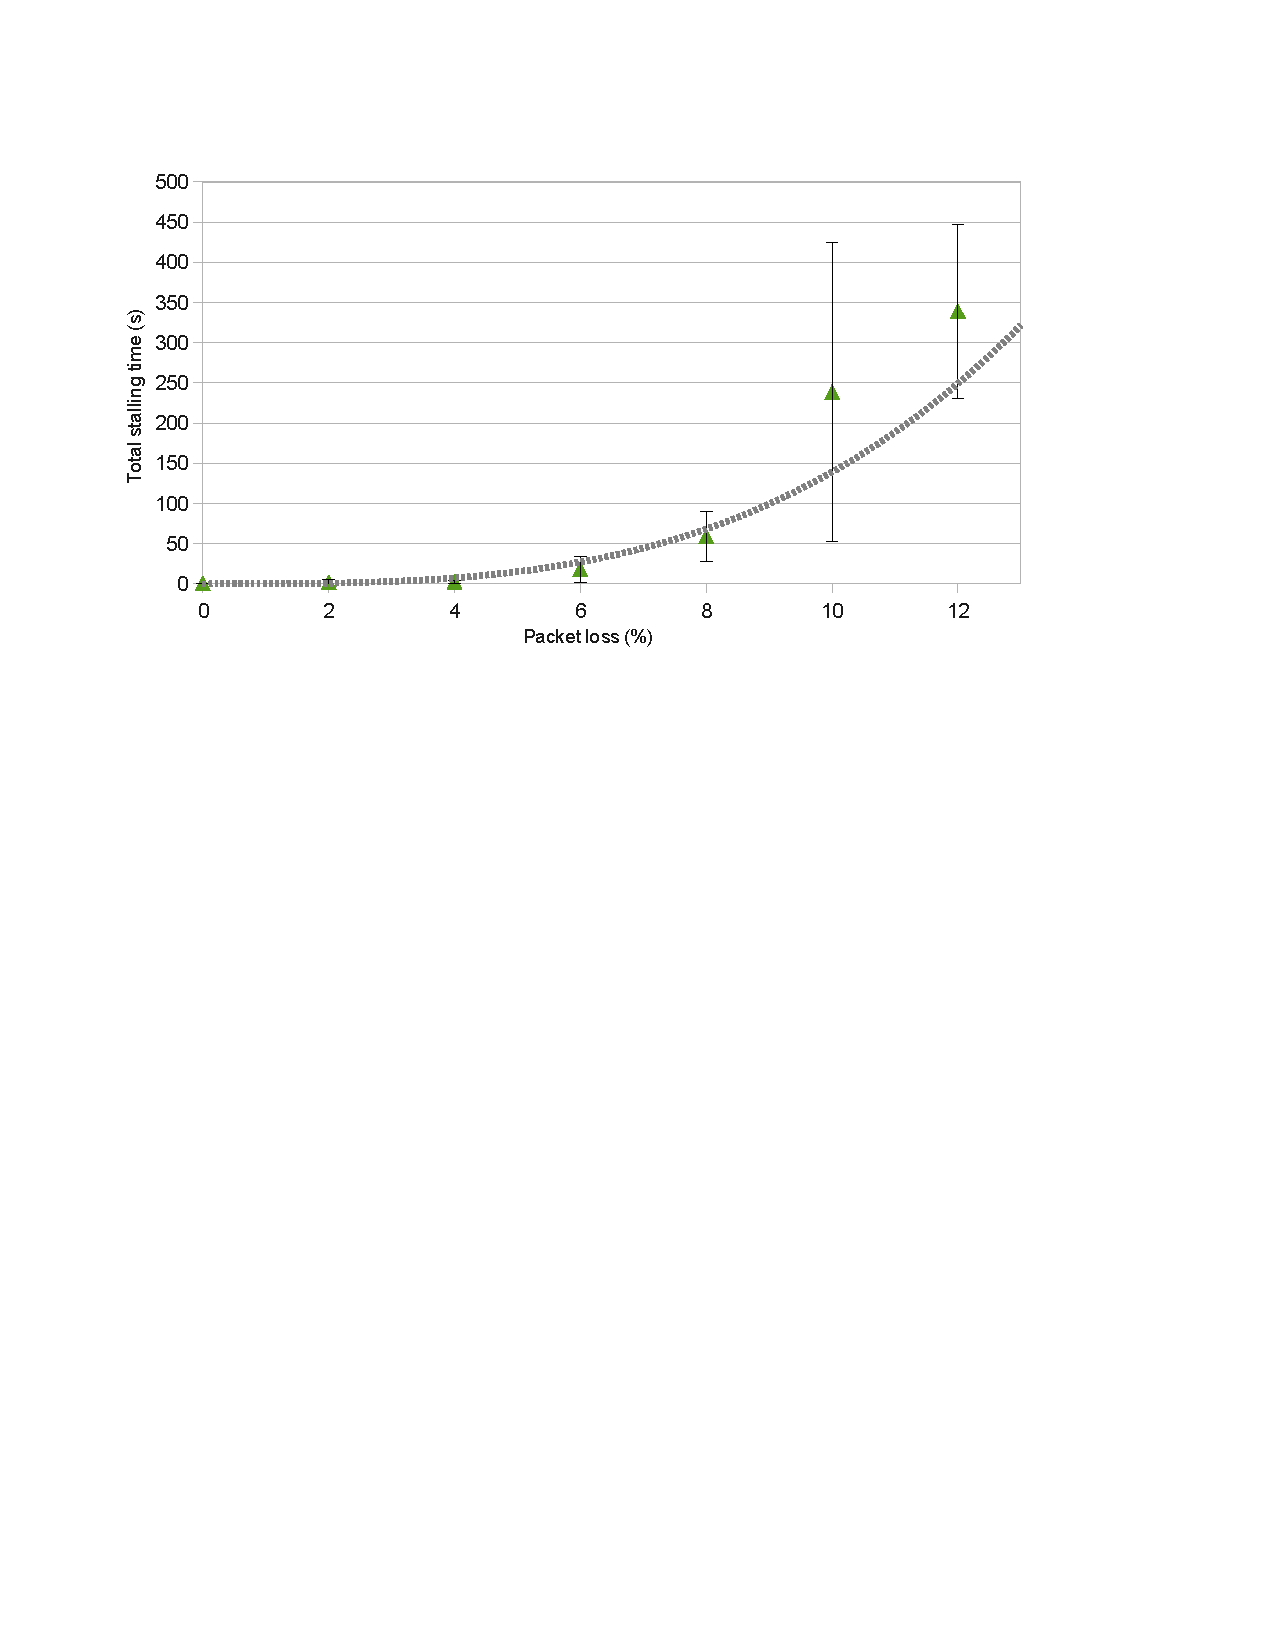
\includegraphics[width=\textwidth]{images/loss.pdf}
                \caption{Loss Graph.}
                \label{c3:fig:lossseries}
        \end{subfigure}
\caption{Total buffering time and exponential trend for degraded network parameter scenarios.}
\label{c3:fig:seriesgraphs}
\end{figure}


%%%%%%%%%%%%%%%%%%%%%%%%%%%%%%%%%%%%%%%%%%%%%%%%%%%%%%%%%%%%%%%%%%%%%%%%%%%%%%%%
\section{Outlook}
\label{sec:outlook}

Streaming to mobile devices, especially in mobility scenarios, arises several new issues not seen at wireline connected devices. The lower-layer protocols on the radio link can cause additional unexpected behavior. Handover between radio cells can cause long periods of very high delay (up to seconds) and packet reordering which does not play well with TCP, resulting in a decreased throughput. Therefore, we would like to investigate its interplay with server-side bandwidth pacing methods as employed by YouTube.

%For the future we plan to extend on these trials to mobile scenarios as well as improve the fidelity of both our model and QoE metric.

We also would like to extend our analysis of video streaming to adaptive HTTP streaming mechanisms previously mentioned. We expect them to further complicate the client's buffer management algorithms but they could also serve as a full replacement and evolution to RTP streaming.




%%%%%%%%%%%%%%%%%%%%%%%%%%%%%%%%%%%%%%%%%%%%%%%%%%%%%%%%%%%%%%%%%%%%%%%%%%%%%%%%
\section{Conclusion}
\label{sec:conclusion}

In our research we analyzed both the topology as well as the streaming performance of the YouTube platform as a popular example for today's Web-based video delivery. 

With the Seattle platform we actively probed the CDN and discovered several geographical and time-dependent features. Through streaming experiments we have shown that packet loss and delay have considerable influence on the quality of the HTTP video delivery but overall it is reasonably robust to conditions in normal wireline networks. Whether they work as well in wireless networks is a question for future research. Furthermore, we looked at various theoretical and real-world buffering models. We observed that one needs to strike a balance between frequency and length of buffering phases to achieve acceptable playback quality. However, quantizing the quality is also a topic for further research.



%albeit for values which probably will not be observable in the wild for wireline network accesses and if providers have sufficient infrastuctures
% however mobile could very well ...

\section*{Acknowledgment}
\label{sec:acknowledgments}

The authors would like to thank Ákos Lukovics, Oliver Michel, Stephan Seebacher, and Bernhard Gruber for their investigation of YouTube’s playback mechanisms, implementations and measurements.



%%%%%%%%%%%%%%%%%%%%%%%%%%%%%%%%%%%%%%%%%%%%%%%%%%%%%%%%%%%%%%%%%%%%%%%%%%%%%%%%
\section{PV2012 YT EMU INSERT}
%%%%%%%%%%%%%%%%%%%%%%%%%%%%%%%%%%%%%%%%%%%%%%%%%%%%%%%%%%%%%%%%%%%%%%%%%%%%%%%%
\section{Introduction}
\label{sec:introduction-PV}

Video streaming resonates well with web users, and streaming traffic makes up an ever-growing share of network traffic. At the same time, multiple streaming methods exists, resulting in a multitude of protocols, codecs, and their variety increases at an astonishing rate. Furthermore, the current boom in smart-phones creates an increasing plurality of access network technologies across which media are streamed.

This poses a problem to traditional analytical approaches like source-traffic modeling: Such models are complex to develop, and hard to adapt to new streaming mechanisms; often, they deliberately omit details for reasons of analytical tractability, or only look at single layers of the network stack.

The method presented in this paper rather aims to evaluate performance by capturing generic behavioral patterns of streaming mechanisms, embracing the perspective of a streaming application. Specifically, we model the level of the playback buffer, and thus can subsume both network and playback behavior, while maintaining flexibility and adaptability with regards to the actual streaming server implementation, type of transmission network, protocol stack, and codec. Our model reports perceivable artefacts of buffer underruns, e.g. skips or stalls, which could then be fed into a QoE model to yield actual user QoE values.\\



% Multiple incarnations of media streaming, but similar and (most of all!) comparable concepts and mechanisms => no need to assess single, specific protocols, networks, codecs, etc., but measure and describe generic, universal, common behavioral patterns => model, compare performance based on behavioral, structural commonalities. Choose for example a (range of) timescale(s) to find sets of mechanisms you need to look at. First use case to show how our system works: Progressive HTTP streaming. Will show adaptability to adaptive streaming and different protocols.


The remainder of this paper is structured as follows. Section \ref{chap:relatedwork} reviews related work. Section \ref{sec:analysis} discusses issues arising from different (and multiple) parts of the network stack. In Section \ref{sec:appbehavior}, we take a closer look at the buffering and playback behavior on both the theoretical and practical side of things. Our testbed approach is described in Section \ref{sec:testbed} and evaluated in Section \ref{sec:evaluations}, where we conduct an exemplary measurement and modeling campaign on the popular YouTube platform. Section \ref{sec:conclusion-PV} wraps up the paper.





%%%%%%%%%%%%%%%%%%%%%%%%%%%%%%%%%%%%%%%%%%%%%%%%%%%%%%%%%%%%%%%%%%%%%%%%%%%%%%%%
\section{Network Stack Layers and Streaming}
\label{sec:analysis}

In network layering models, it is often assumed that the layers are independent (or at least strongly decoupled) from, and only present narrow interfaces to, one another. From a conceptual point of view, media streaming is a process governing the application layer. Thus, the application and its behavior might be thought to dominate the overall streaming process and associated quality. In this Section, we will show that this is not necessarily the case. % for reasons of conflicting time constraints on the different layers, 


Figure \ref{c3:fig:timescales} overviews the approximate time scales on which activities on different layers may take place, spanning a remarkable range of twelve orders of magnitude. Multiple layers might implement the same or similar functionality, e.g. flow control in the application and on transport layer, resulting in nested control loops, which might be coupled due to the timing constraints. 


% As such, the aim of this deliverable is to provide a methodology that identifies influencing factors on the user experience, and quantifies the relative impact of these factors.


\begin{figure}[htbp]
	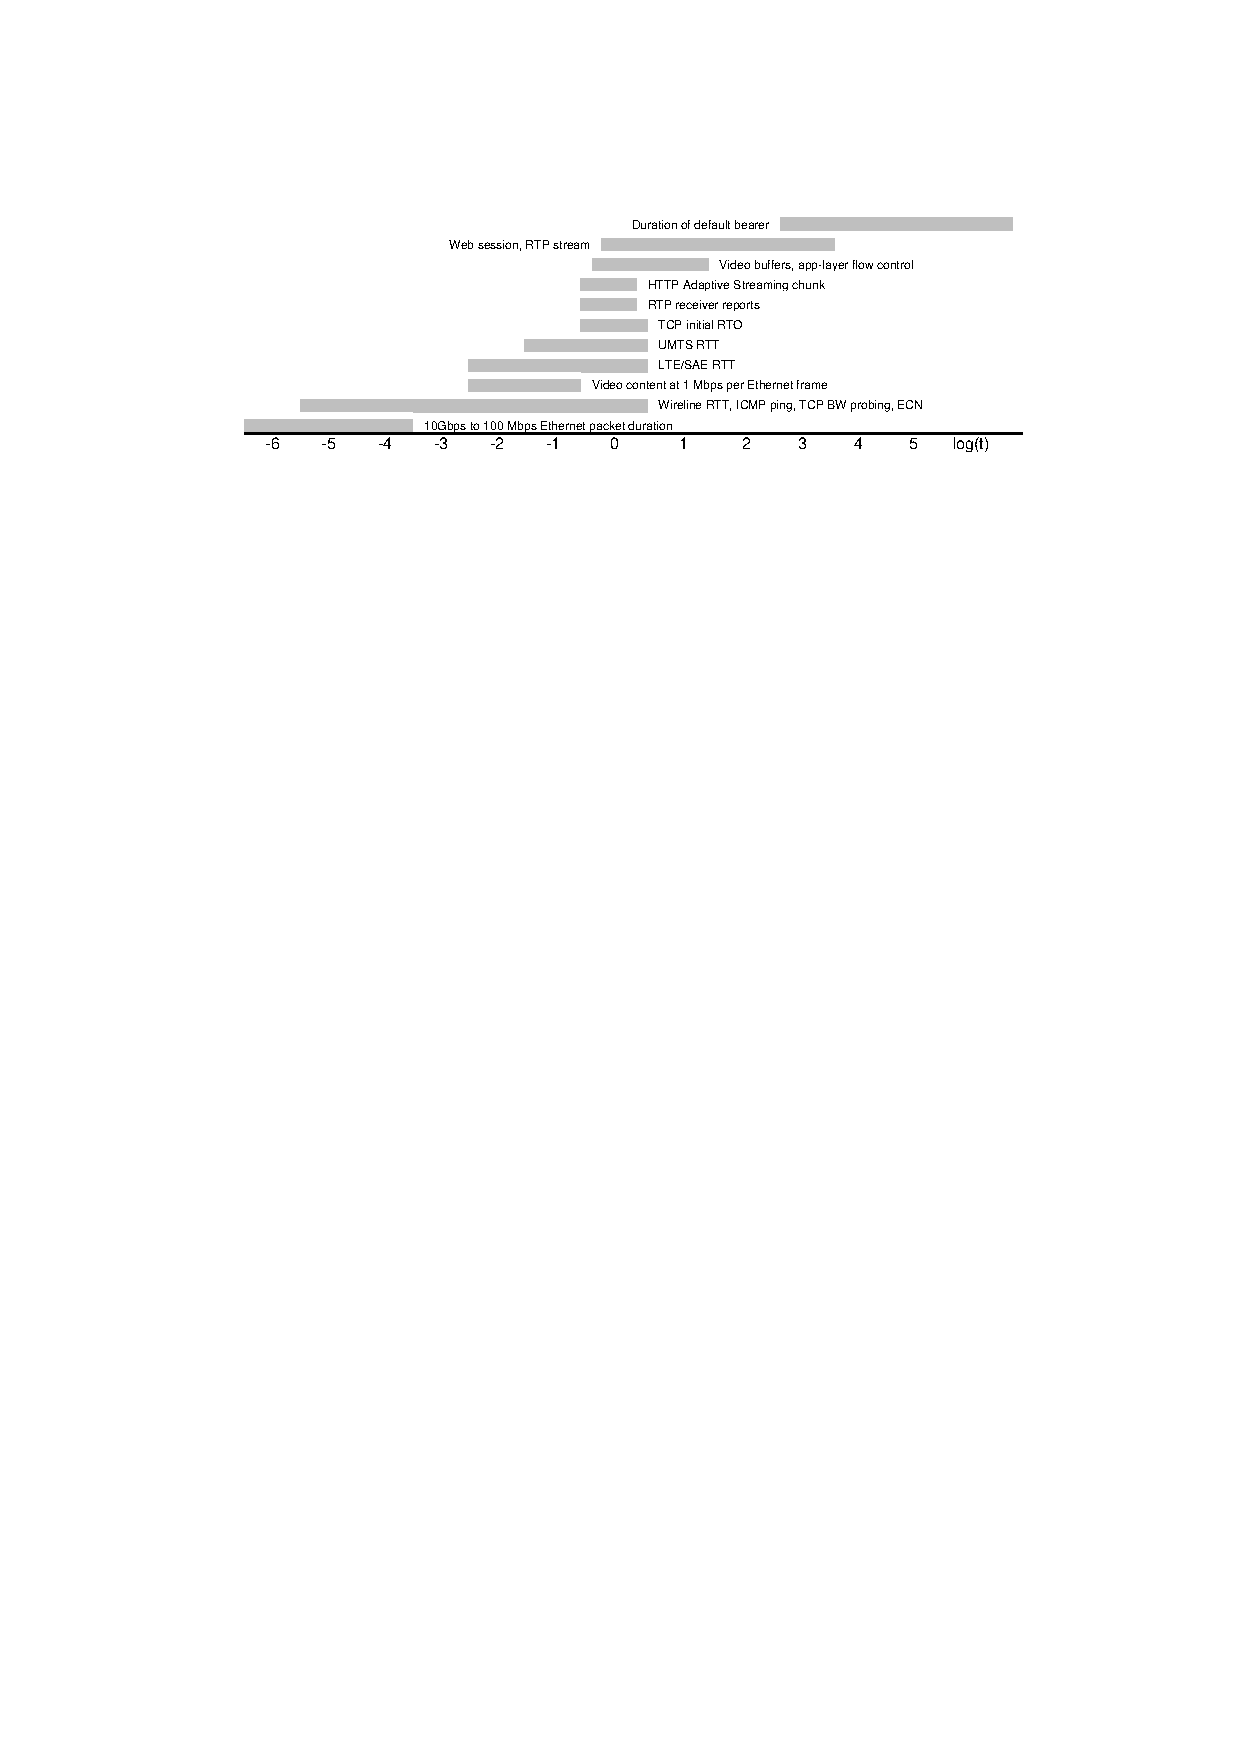
\includegraphics[width=\textwidth]{images/timescales.pdf}
	\caption{Relevant time scales in the layers of the stack}
	\label{c3:fig:timescales}
\end{figure}



\subsection{Network Layer}

As seen in Figure \ref{c3:fig:timescales}, the time constants found in different network implementations range from nanoseconds (for Gigabit Ethernet) to seconds (for UMTS and LTE/SAE wireless networks), depending on the technology used. This also influences the achievable round-trip time across such networks, which directly affects the performance of higher-layer protocols: IP, ICMP, UDP, TCP, and subsequently all application-layer protocols are all subject to these timing constraints.

In the case of wireless networks, typical effects of wireless connectivity relating to physical phenomena like fading and interference come into play. Flaky radio connectivity is a major source of packet loss and excessive delay. Certain cellular mobile technologies like UMTS and its evolutions implement loss concealment themselves, confounding IP's assumption of a host-to-network layer lacking guaranteed delivery. Other peculiarities of cellular mobile networks include a maximum transmission unit (MTU) opaque to IP, and delay variances as functions of packet sizes \cite{Arlos10} and radio access technologies \cite{laner2011dissecting}.


% Then, the technological progress enables both handsets and the network to become faster: Compar-ing the delay budgets given by [ANDE] for UMTS (2005) and [KESS] for HSDPA R99 (2009) respectively, it is seen that the delay caused by pro-cessing on the mobile terminals decreased by a factor of 30, and that the core network has become faster by an order of magnitude as well. [SVOB] has additional information on the delay budgets per network entity, varying the packet size as the parameter.
%LTE/SAE also makes heavy use of the concept of bearers, a type of tunnel through the mobile network associated with quality levels and policy control. Although the bearer concept already exists in UMTS, operators seem cau-tious to configure other bearers than the default one, and support by hand-sets is not widespread either. The process of setting up LTE bearers is specified amongst others in [3GP23]. The setup procedure is sufficiently lengthy to be measurable and influence packet delay on initiating connec-tions [FIED]. Analyzing the effects of bearers on user data flows is the sub-ject of the Ursa Major project [URSA] at the University of Vienna with the FTW.
%
%For reasons of radio spectrum efficiency, applications with long patterns of inactivity may be scheduled to not use HSDPA. This also causes measura-ble additional delay for applications [SVOB and their references 3 and 4].
%


\subsection{Transport Layer}

%As detailed in Section 3, the application and associated application-layer protocols dictate certain requirements on the transport protocol to be used.

The two most widely used transport protocols are TCP (Transmission Control Protocol) and UDP (User Datagram Protocol). As is widely known, TCP implements a number of elaborate mechanisms to establish and tear down connections, deliver data to the application in sequential order, conceal loss on the network layer, adapt its bandwidth usage to the capabilities of the other endpoint (flow control) and the network (congestion control), and share bandwidth fairly through a distributed control algorithm. Furthermore, its notion of ports adds a layer of addresses on top of the network layer.

UDP also supports port numbers, but does not include any of the other mechanisms TCP has. This spurs the common misconception that UDP is the faster transport protocol. In fact, all packet types are subject to the same round-trip time, independent of the transport protocol used. Delays in the delivery of data to the upper layer occur in TCP when segments are considered lost in transmission (via timeouts or gaps in the range of acknowledged segments). TCP retransmits the lost segments, causing the round-trip time to spike temporarily. In the case of UDP, the application layer handles (or ignores) packet loss.

As indicated in the previously, mobile cellular networks often conceal packet loss, which is used by TCP as an indication for network congestion. Rather than lost, packets are highly delayed, which can cause sub-optimal bandwidth usage. Mobile networks also show artifacts relating to port and network address translation (commonly subsumed under ``NAT''), firewalling, and middleboxes interfering with TCP timeout on long-lived connections \cite{wang2011untold}.


%It must be noted that the loss of acknowledgements can usually not be discriminated from actual packet loss, and 
%
%nor does its assumption of loss hold in the face of highly varying delays, i.e. jitter, as typically found in mobile networks.

%There are lots of controls for mobile operators to engineer traffic flows in their networks. In \cite{wang2011untold}, the authors show artifacts relating to port and network address translation (commonly subsumed under “NAT”), firewalling, IP address assignment etc. Operators can also employ traffic engineering on backhaul links, and use policies to better support (or regulate) specific services for specific users or user groups, schedule traffic at different times of the day, etc.



\subsection{Application Layer}

There exists a diversity of streaming applications and associated application-layer protocols, each supporting to differing degrees certain types of streaming, and each having its own set of requirements, depending on the content type (pre-generated or live), the codec and its bitrate, and playback control and quality feedback.

One classification for streaming protocols might be their body of standardization: There are many proprietary protocols with undisclosed or legally restricted standards documents, e.g. RTMP (Real Time Messaging Protocol) and RTMPCS (RTMP Chunk Stream), MMS (Microsoft Media Server), and WMSP (Windows Media HTTP Streaming Protocol). Other protocols and protocol families are standardized by open bodies such as the Internet Engineering Task Force (IETF). In our work, we focus on these ``open'' protocols.

In the latter category are two well-known protocol families for media streaming, Real-time Transport Protocol (RTP) and Hypertext Transfer Protocol (HTTP). RTP sees most of its use in walled garden services such as IP TV. HTTP is the single most common application layer protocol on the Internet, owing its popularity to the ubiquity of web browsers. As RTP is designed for media transport, a companion protocol suite consisting of RTCP (for control information), RTSP (for stream control like pausing), and SDP (for session management) is often used. RTP is mostly transported using UDP.

In contrast to RTP, HTTP was not designed for specific payload types apart from HTML. The actual streaming protocol behavior is defined by the application, not by the protocol. Every service is thus free to define its own distinct protocol behavior. For HTTP, many de-facto variants for streaming exist, but many if not most are not formally standardized. There is work underway in the IETF to create a standard for Dynamic Adaptive Streaming over HTTP (DASH).



% Within these protocol families, a multitude of implementations exist that suit specific demands. RTP specifies an initial set of profiles (RFC3551), with a multitude of definitions cropping up with every new type of media coding scheme . In HTTP, the actual transfer model, addressing, and metadata mechanisms have been in place virtually unchanged since 1999, when HTTP/1.1 was specified. Much innovation has since gone into the payloads transferred via HTTP, as well as the control of its underlying transport protocol, TCP.

% Both protocol families offer a wide range of techniques, established and recent, de-facto and formally standardized, each supporting different types of streaming and content, and each subject to the interplay of content requirements, the application, the network, the media player, the layer stack, etc. Seemingly, not one single protocol can solve all problems at once. % Let’s now look at the specific properties of RTP and HTTP.


% The Real-time Transport Protocol (RTP) [RFC3550] is an IETF protocol designed for (near) real-time payload such as multimedia or sensor data. It is designed for support by the network. RTP supports mixers and translators that enable transcoding of content as it travels through the network.

% Since RTP is typically transported over UDP, it is also multi-cast compatible. For example, A1 Telekom Austria’s A1 TV uses an Organization-local cope Multi-cast [RFC2365] tree with distinct IP addresses for each program. At the same time, UDP is not inherently congestion-controlled, and RTP’s own congestion control mechanism (if activated at all) has a relatively long delay to respond for reasons of rate limiting on the control channel (see [RFC3550, Sec. 3.5.1] for details). This means a wide-spread use of RTP could even cause congestion collapses in parts of the network.

% RTP employs a server-side control scheme. This means that the server is responsible for every aspect of the streaming process. Even client play and pause requests are directly communicated to the server. Therefore the server also has to maintain a session for the user.




%In contrast to RTP, HTTP streaming facilitates complete client side control. HTTP includes some support by the network in the form of proxies, but there are signaling methods that can e.g. forbid the caching of specific content through the no-cache directive [RFC2616, Sec. 14.9.1].
%Due to its use of TCP as the transport protocol, HTTP has issues with inter-activity, especially across lossy links.
%3.2	Protocol Comparison
%In Figure 3, we compare the properties of three specific implementations of streaming protocols, namely RTP with RTCP, progressive HTTP, and adaptive HTTP. In RTP streaming, it is customary to have multiple flows for different parts of the media stream, e.g. audio and video, and a separate control connection. In HTTP, one (or multiple consecutive) TCP connection is used for both control and data transfer.
%In RTP, flow control on the transport layer needs to be done by the server application. The same goes for congestion control, which is implemented us-ing receiver reports, or might be left out altogether. HTTP uses TCP as its transport protocol, and thus inherits its flow control and congestion control features.
%There are several implementations for application-layer flow control. Figure 4 shows an overview on basic and modern flavors. Simple bulk transport is the typical web download model, which assumes that both the client and the server try to transfer the data as fast as possible. Contrarily, paced transfer is implemented by RTP, where the server sets the bitrate the client will see. An interesting variant on paced transfer is paced block transfer, implement-ed for example in the YouTube block sending mechanism [METZ]. The specific incarnation consists of server-controlled burst sending of 64kB blocks and inter-block gaps of variable length to adjust the download rate to the average video bitrate. An additional initial burst phase is present to prefill buffer. The method is observed in detail in [ALNE11].
% 
%Playback control is actually done by the server in the case of RTP, where the client issues requests to, e.g., pause the stream, and the server then reacts. In HTTP, the client is in much stronger control of the playback, and need not notify the server of a user’s decision to skip backwards, etc. 
%For the exchange of transport control information such as packet loss, RTP uses a companion protocol named Real-Time Control Protocol (RTCP). HTTP again leverages TCP, where such information is exchanged implicitly. It must be noted however that due to the flexible data format RTCP pro-vides, more concise information can be signaled in addition to transport control related matters.
%To conclude, the different protocols are also specified to different degrees. As stated before, there is a large body of RFCs relating to RTP and its adaption to new media, content, etc. For HTTP, many de-facto used variants adapted to streaming exist, but many if not most are not formally standardized. There is work underway in the IETF to create a standard for Dynamic Adaptive Streaming over HTTP (DASH) .
%



%%%%%%%%%%%%%%%%%%%%%%%%%%%%%%%%%%%%%%%%%%%%%%%%%%%%%%%%%%%%%%%%%%%%%%%%%%%%%%%

\subsection{Application Behavior}

The time scale on which streaming applications buffer content lies in the range of seconds. This is a necessity in a best-effort network, as the available network bitrate might drop unexpectedly and could drain a shallower buffer quickly. % On the other hand, given sufficient band-width or even bandwidth guarantees as demanded in SAE, buffer sizes could be reduced, improving interactivity of the stream and enabling closer-to-realtime live streaming or conferencing.
The application behavior represents a trade-off between different types of perceivable artifacts -- initial startup delay, stalls, (partial) media skips (e.g. continuous audio, but skipping video), and quality adaption. The next Section will specifically look at these issues.




%%%%%%%%%%%%%%%%%%%%%%%%%%%%%%%%%%%%%%%%%%%%%%%%%%%%%%%%%%%%%%%%%%%%%%%%%%%%%%%%
\section{Application Behavior}
\label{sec:appbehavior}

%This section provides an analysis of different playback models, both hypothetical best/worst-case, and actually implemented ones. We set off to develop a generic model for the playback process of a streaming application, and then explore the result space yielded by the application behavior.
%
%\subsection{Generic playback model}

To play back a media stream, an application needs to maintain a media buffer of sufficient size to at least gather enough data to reconstruct one single atomic unit of playback such as a video frame.

The current buffer level at time $t$ is given by the amount of data received from the network so far, diminished by the amount of data already played back. The actual media format used in the stream determines the progress of the playback process, whereas the network conditions and application download strategies yield the overall progress of data reception:

\begin{equation*}
\mathit{buffer}(t) = \sum_{0}^{t} data_\mathrm{received} - \sum_{0}^{t} data_\mathrm{played}
\end{equation*}
 
The playback buffer level governs how well the player can conduct the playback. If the buffer reaches zero size the playback process stops and stalling occurs. Then a decision is required when to restart the playback process again after a stall, and if the stream should skip forward to a more current playback position. This process is the core part of the playback model for an HTTP streaming service. The model could also be extended to accommodate adaptive streaming mechanisms that feed back the buffer level to influence the download strategy of the player, e.g. send a receiver report to request a lower-bitrate stream in the case of RTP. % Consequently, the progress of data received would increase at a lower rate, and the playback rate would decrease as well once the residual stream data in the buffer were played out.

Playback models need to define the behavior at the occurrence of one of two conditions during the playback process. These are the initial playout delay (the point in time when to start draining the playback buffer), and the buffer fill level at which to start playing again if the buffer had intermittently emptied and the video had to be stopped.

These decisions yield a stalling period distribution for a streamed video. The frequency and the duration of stalls directly relate to the decision function of the playback model. The more frequent the stalls are, the shorter they will be; if the function produces longer stalls, they will be less frequent.

There can be other parameter spaces governed in the model. For example, in a live streaming scenario a user could prefer to always stay at the most current stream position. To enable this, a player would skip older parts of the video. If the user prefers to consume the entire stream, the player would show the video without skipping parts, but pause intermittently. 

Another user parameter is the quality level of the video for adaptive streaming. This trades off between maintaining a certain quality level and putting up with increased waiting times, and dropping the quality to a level sustainable at the current transmission rate.

%\begin{figure}[!t] % use 1.75in each for single-column
%\centering
%\includegraphics[width=0.8\textwidth]{usersatisfaction}
%\caption{User Experience as a trade-off between stalls and start-up delay}
%\label{fig:stalltradeoff}
%\end{figure}

% As sketched for the start-up delay and the number of stalls in Figure \ref{fig:stalltradeoff}, all of these resulting parameter spaces could in turn be mapped to user satisfaction metrics describing the user's experienced quality. 
% However, this mapping goes beyond the scope of this work. The focus is rather on the creation of simple evaluation methods to assign combinations of network conditions and playback models to specific stalling characteristics defining a base for user satisfaction decisions.

The next subsections present four stalling playback models, ranging from theoretical models that represent boundaries to the values possible in stalling characteristics, to the Firefox and the Flash model, which represent actual player behaviors that can be seen ``in the wild''.


\subsection{Simple Playback Stalling Model}
The behavior can be summarized as ``Whenever anything can be played from the buffer, do so''. This means that, if the player is currently stalling and a complete frame becomes available in the buffer, playback will immediately restart and the frame will be shown even if this means stopping playback after that frame again. This results in the lowest required buffer space. Moreover, it gives an upper limit for the number of stalls occurring\footnote{As a video frame is atomic, no other model could possibly stop the playback more often.}.

\subsection{Initial Playback Delay Model}
The model is similar to progressively downloading the whole stream, as it will simply delay the initial start of the video until it can be played completely without any buffer underruns occurring. The only stall occurring is the initial waiting period until the video starts. The time spent waiting will also be minimal. The downside of this model is its use of perfect knowledge on the future network conditions at any point in time, making it purely theoretical. Actual streaming players need to accurately predict the transmission process, e.g. through moving averages.


The stalling and initial delay models define the maximum achievable upper and lower limits for the stalling parameter space for all possible real models.


\subsection{Firefox HTML5 Model}
The algorithm used in the Firefox 4 browser is an approximate realization of the HTML5 video standard \cite{html5} which suggests starting the playback only when it can be ensured that the video can be played without interruption similar to the initial playback delay model.

The algorithm and its variables are shown in Algorithm \ref{c3:alg:firefox-PV} and Table \ref{c3:tbl:buffvars}, respectively. Firefox 4 uses moving averages to estimate the development of the transmission rate. It does not differentiate between intermittent and initial conditions. As the approach is similar in concept to the initial playback delay model, %it results in a very large required buffer space, but also %
it sports very few stalling events due to conservatively chosen (i.e., long) buffering times.



\begin{figure}[htbp]
	\centering
	\begin{algorithmic}
		\IF {$s_{MA} > v_{MA}$} 
		  \STATE $c \gets ( b_b=20s \lor b_T=20s )$
		\ELSE
		  \STATE $c \gets ( b_b=30s \lor b_T=30s )$
		\ENDIF 
	\end{algorithmic}
	\caption{Firefox playback (re-)start decision algorithm.}
	\label{c3:alg:firefox-PV}
\end{figure}


\begin{table}[htbp]
	\caption{Variables involved in buffering decisions.}
	\label{c3:tbl:buffvars}
	\centering
	\begin{tabular}{|c|c|} \hline
	Variable & Explanation \\ \hline\hline
	$s_{MA}$ & Moving average of the transmission speed. \\ \hline
	$v_{MA}$ & Moving average of the video bitrate. \\ \hline
	$c$   & Condition upon which to start/resume playback. \\ \hline
	$b_b$    & Amount of video data the buffer contains. \\ \hline
	$b_T$    & Amount of time spent in non-playing buffering state. \\ \hline
	\end{tabular}
\end{table}
 
  
\subsection{YouTube Flash Player Model}
This model is facilitated by the Flash Player used by the YouTube website. It will initially start the playback after it has buffered two seconds of video data. If a stall occurs it will restart playing after five seconds of video are in the buffer.
The Flash Model assumes sufficient network conditions in the beginning, requiring only a short initial playback delay to pre-fill the playback buffer. If, however, stalling occurs, then it will buffer longer to keep the stalling frequency down.


%\subsection{Further Models and Variables}
%In general, every streaming service practically implements its own playback model. Most of them will be very similar to the presented ones as the choices and parameters a streaming player has are rather limited.

%For simple TCP streaming, the client can only influence the playback start and restart points after stalls. Adaptive streaming, i.e. streaming with the possibility of rate adaptation during playback, adds the choice of the quality and the number of segments to request in advance to control the fill level of the buffer.

%Typical models for simple streaming will often try to set the current rates of the streaming transmission and the video in comparison to estimate if the buffer will continue to drain or fill. Depending on this variable an optimal buffering length can be calculated. The size should typically be larger if the transmission rate is not sufficient enough for the playback process to prevent frequent stalls.



%%%%%%%%%%%%%%%%%%%%%%%%%%%%%%%%%%%%%%%%%%%%%%%%%%%%%%%%%%%%%%%%%%%%%%%%%%%%%%%%
\section{Testbed Architecture}
\label{sec:testbed}

Testing and comparing new protocols is a complex and time-consuming undertaking if traditional evaluation approaches such as analytical source-traffic models are employed. For today's fast-paced development of streaming protocols, faster evaluation methods are needed. A testing environment must be simple and sufficiently flexible to allow its application on and adaption to current and future protocols, services, network structures, and associated parameter spaces. 
% This also demands to take a generic approach that does not rely on specific implementations. 
At the same time, it must be able to answer specific questions about  protocols, applications, and network setups. Finally, the results yielded from analyzing and evaluating a streaming service should be user-oriented, i.e. provide a foundation of data that can be fed into the calculation of a Quality of Experience (QoE) model. We believe our proposed testbed, the architecture of which will be explained in the following, meets these requirements.

%In the following sections, we first describe the methodology and then present exemplary evaluations to show how this approach can be used to evaluate real world streaming scenarios under configurable network conditions. 
% Through configuration, one may evaluate the influence of network parameters, states, and topologies on the multimedia stream, e.g. parallel bearers with different quality settings, cross traffic, or stream-support middleboxes.


Figure \ref{c3:fig:testbed} depicts the evaluation testbed. % To enable rapid comparison of network quality of service against application behaviors we employ a two-step process. 
Conceptually, it replicates the actual steps a user would perform to consume a media stream on a playback device. Through appropriate configuration different scenarios can be modeled, e.g. network conditions, behavior and specifics of the user device.
 
 
\begin{figure}[htbp]
	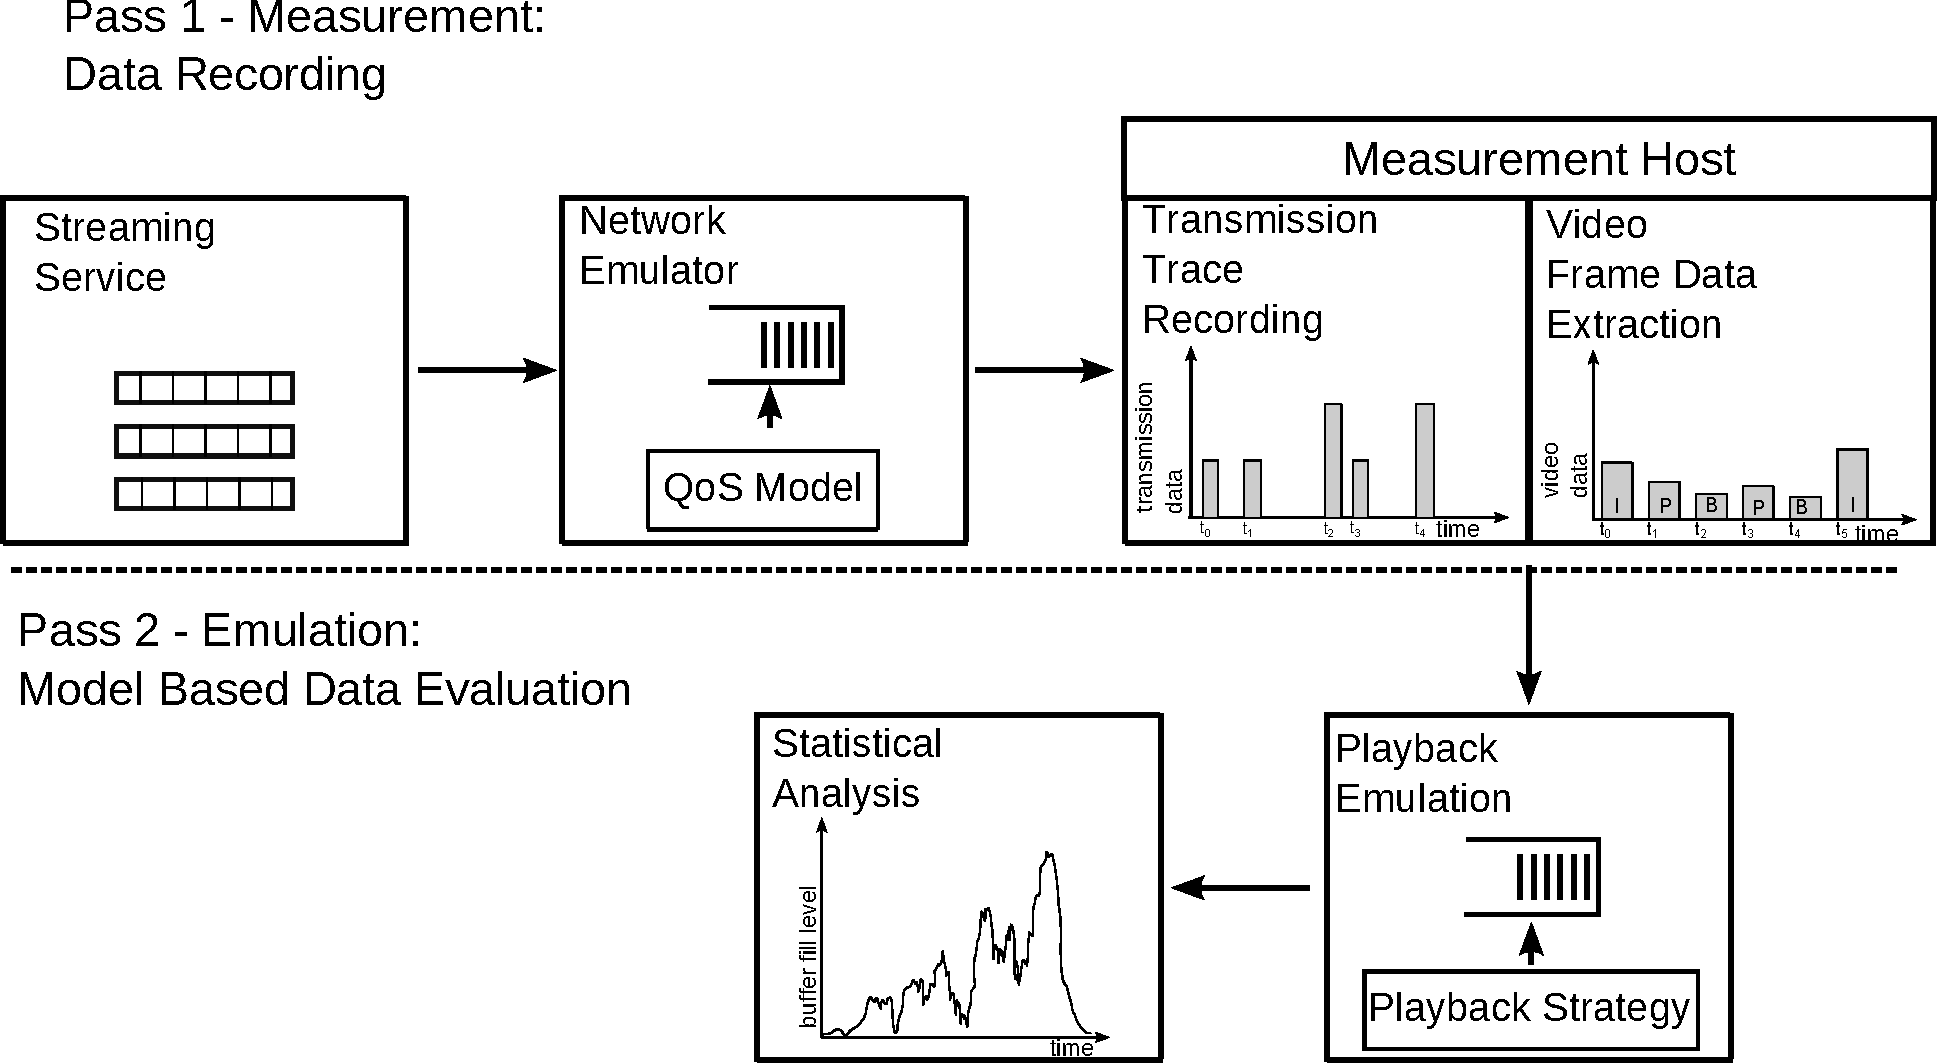
\includegraphics[width=\textwidth]{images/measurement-model.pdf}
	\caption{Testbed Schematic.}
	\label{c3:fig:testbed}
\end{figure}

In the first pass of the process, the stream data is transmitted from a server to the client. The server can either be an actual streaming service on the Internet, or a local server (to eliminate the unpredictable impact of the Internet connection). The traffic is directed through a network emulation node capable of altering the network QoS parameters, i.e. latency, jitter, and packet loss. The parameters could also be set according to stochastic models derived from actual network traces. 
%Therefore, almost any kind of access network conditions can be modeled. 
%Of particular interest are mobile radio behaviors and core network architectures. An example would be to compare guaranteed bit rate (GBR) with best-effort PDP contexts to assess the impact of QoS parameters on the stream quality.

The measurement host downloads and records the video stream as a network trace. For HTTP streaming, it issues a single HTTP \texttt{GET} request on the video file, and then maintains the TCP connection until the file has fully arrived. A trace should at least contain the sizes and timestamps of every incoming packet. More detailed traces can be used to scrutinize other layers of the connection, e.g. the dynamics of TCP receive window size. The packet trace is then decoded using the popular open source \texttt{ffmpeg} suite, yielding another set of traces consisting of video frame sizes and playout timestamps.

In the second pass, these two traces are then used to feed the playback models described before. The playback emulation process combines the transmission and video frame traces to calculate the playback buffer fill level for every point in time during the playback. It then generates statistics about user-perceivable artifacts such as playback stalls that would occur during the playback. These statistics can then be compared to the results of other models and network QoS.

% For simple HTTP streaming, there is no feedback from the client to the server that would result in adaptions of the stream (``rate control''). Therefore, recording the packet trace and simulating playback are decoupled, as the latter cannot influence the former. As such, the testbed can test and compare several playback models on the same recorded network trace. This enables fast and efficient comparison of non-feedback protocols subject to the same network conditions.


\section{Evaluation}
\label{sec:evaluations}

The results presented here show some of the capabilities in comparing play network conditions based on playback models. We compare how the four playback models introduced previously fare against each other in a measurement series featuring  emulated transmission latency and packet loss . At the same time, we acknowledge that other specific questions are not touched in this first set of experiments, e.g. the inclusion of a mobile network or handset, or RTP-based streams.

The video used in our measurements was streamed from the YouTube web site. This provides a realistic base for all the experiments. Note that YouTube also employs its own form of application layer flow control in addition to TCP's \cite{alcock2011application}. % The influence of the access bandwidth can mostly be neglected with this mechanism as long as the limit is well above the video bitrate, which was the case here.
Details on the streamed video are available in Table \ref{c3:tbl:videoparams}.

\begin{table}[htbp]
	\centering
	\caption{Test Video Parameters}
	\label{c3:tbl:videoparams}
	\begin{tabular}{l|r}
	Video Duration	& 01:32.536 minutes \\ \hline
	Size & 9.61 MiB \\ \hline
	Framerate & 23.976/s \\ \hline
	Average Video Bitrate & 871 Kbps \\ \hline
	Codec & AVC+AAC \\ \hline
	\end{tabular}
\end{table}

For the loss experiment series, the network emulator was configured to drop a certain percentage of packets based on a normal distribution on both the uplink and the downlink direction. There was no loss correlation involved, the existence of which one would expect, e.g., in wireless networks. One streaming run for every two percentage points of additional loss up to 14\% was conducted.
In the latency series, the emulator delayed the delivery of every packet for a set constant amount of time. Half of the total amount is added to the uplink the other half to the downlink. One experiment was conducted for every 100ms of additional delay, up to a total of 5000ms.

After the traces were recorded, every playback model was applied to all runs. For every model, two data points were computed. First, the total stalling time was calculated. This is the time the player keeps buffering and not playing the video, including the initial start delay. To attain results comparable to the other measurements, the stalling time is calculated relative to the total video length instead of an absolute value. The second resulting value is the number of times the video stops playing including the initial delay, i.e. the stalling frequency. Both of them are an indicator how well the playback mechanism can cope with the currently emulated network setup. They could for example be used to either check if a modification to a network has a noticeable impact on streaming experience, or to find an optimized player behavior for a given network.

All models will generally work very similar in good network conditions. If sufficient bandwidth is available, they will play videos with almost no delay and  intermediate buffering. If, however, the achievable TCP goodput is close to the average video bitrate, the buffer may be strained by short deviations from the average rates. %TCP goodput can also be severely limited by high latency and loss. Many TCP congestion control algorithms depend on the round trip time. If the RTT is high, the congestion window will increase much slower.

High latency can also trigger TCP timeouts and retransmissions, and in turn decrease the congestion window, further impacting the goodput. The latency measurements are depicted in Figure \ref{c3:fig:eval-latency}. The stalling time increases with the additional latency. The Initial Start Delay model provides the best possible result in terms of pure stalling time. On the other hand, Figure \ref{c3:fig:eval-latency-numstalls} shows the Stalling model provides always the worst result for the number of stalls. Any other model will lie beyond that line. The Flash and HTML5 models both run in just a few buffering events which however tend to increase in length with rising latency. Attributed to the simple and optimistic assumption of the Flash model, stalling time is usually lower than with HTML5, at the cost of slightly more buffering events.
 

\begin{figure}[htbp]
	\centering
    	\begin{subfigure}[b]{1.0\textwidth}
            \centering
            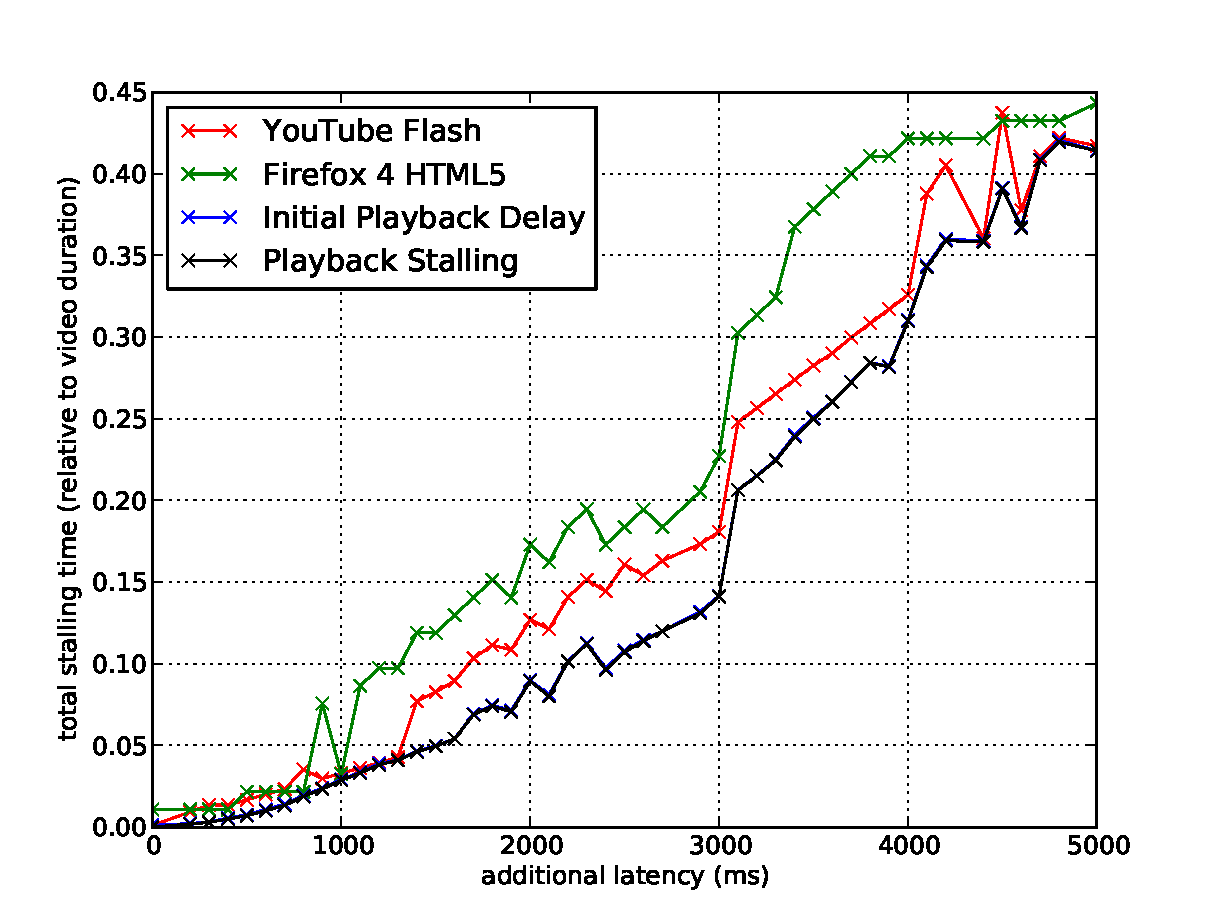
\includegraphics[width=\textwidth]{images/eval-latency-stallingtime.pdf}
            \caption{Total stalling time.}
            \label{c3:fig:eval-latency-stallingtime}
        \end{subfigure}

    	\begin{subfigure}[b]{1.0\textwidth}
            \centering
            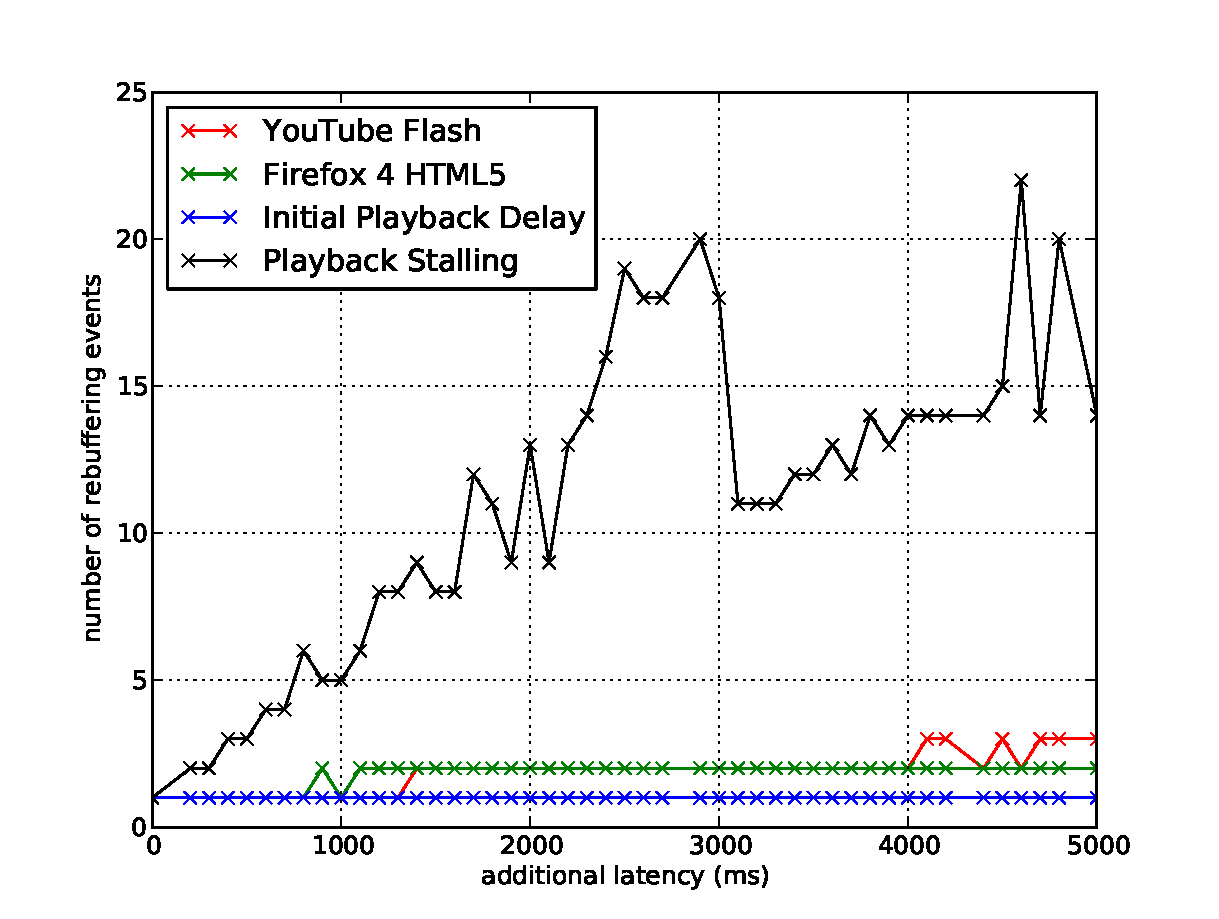
\includegraphics[width=\textwidth]{images/eval-latency-frequency.pdf}
            \caption{Number of stalls.}
            \label{c3:fig:eval-latency-numstalls}
        \end{subfigure}
	\caption{Playback model observations on additional latency.}
	\label{c3:fig:eval-latency}
\end{figure}


TCP goodput is even more severely affected by packet loss. A lost packet results in a duplicate acknowledgement, retransmissions, and a decrease of the congestion window. The problem gets worse if also the ACKs are lost and the connection stalls on missing old segments without which the playback cannot proceed. Figure \ref{c3:fig:eval-loss} shows some exemplary measurements for a loss scenario. While additional packet losses of up to four percent seem to have no noticeable impact on streaming quality, the total stalling time suffers a large increase for any model as seen in Fig. \ref{c3:fig:eval-loss-stallingtime} rendering any streaming attempts practically unusable. Figure \ref{c3:fig:eval-loss-numstalls} shows the extremity of the Stalling model compared to other models reaching a number orders of magnitude larger than any other model.
As a result, when planning a network for streaming applications, the maximum loss should be kept below the noticed mark to achieve reasonable streaming quality. 


\begin{figure}[htbp]
% used yt-delay/hPUGNCIozp0_delay_100 2, spyder with matplotlib config patch
	\centering
    	\begin{subfigure}[b]{1.0\textwidth}
            \centering
            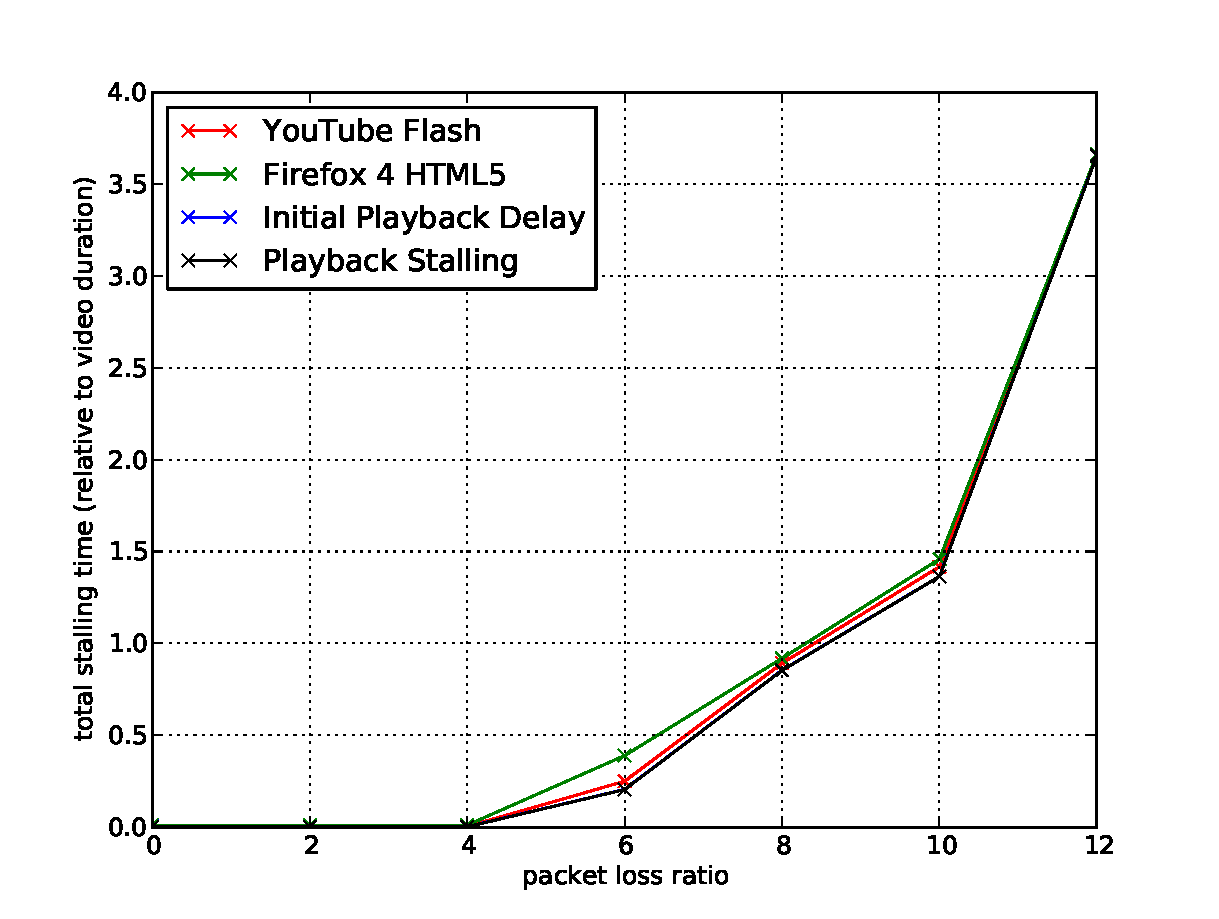
\includegraphics[width=\textwidth]{images/eval-loss4mb-stallingtime.pdf}
            \caption{Total stalling time.}
            \label{c3:fig:eval-loss-stallingtime}
        \end{subfigure}

    	\begin{subfigure}[b]{1.0\textwidth}
            \centering
            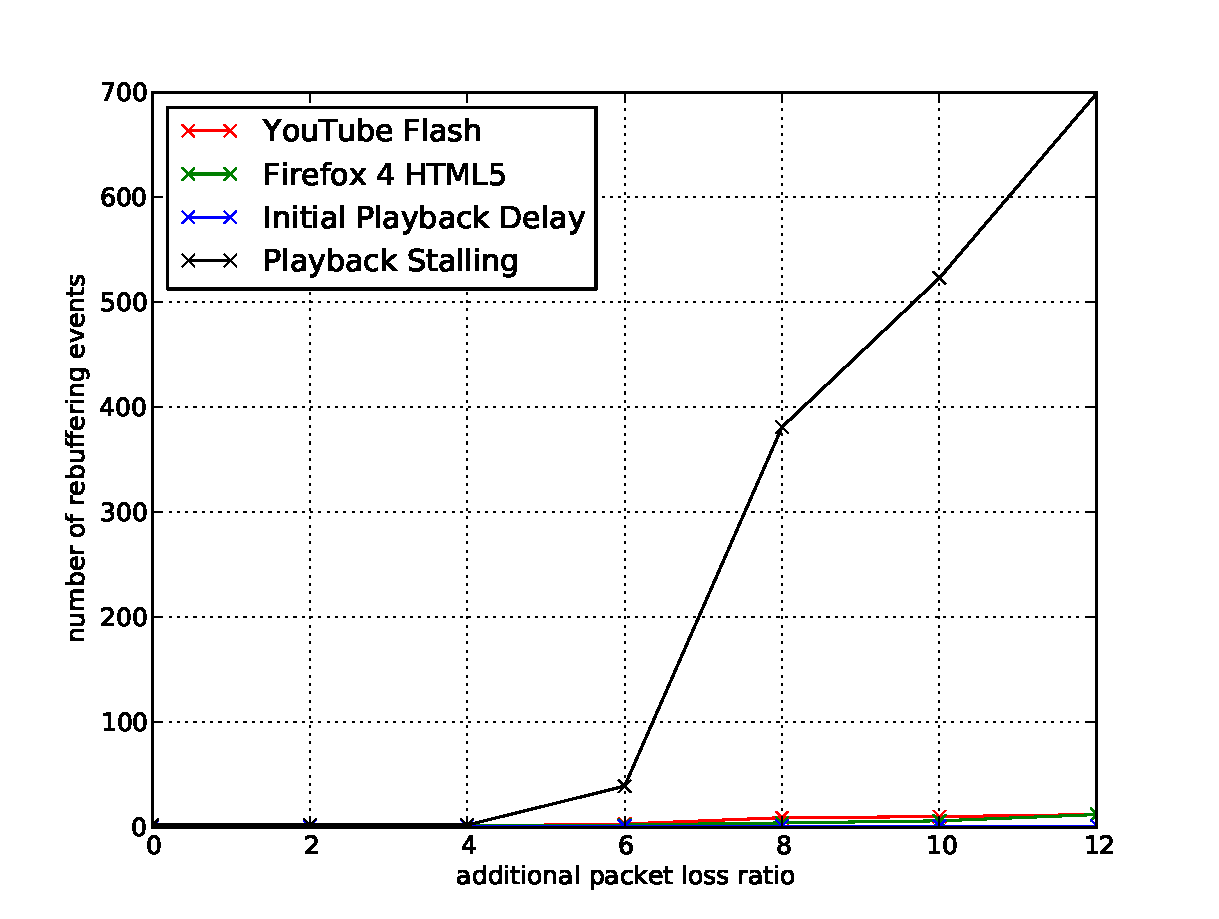
\includegraphics[width=\textwidth]{images/eval-loss4mb-frequency.pdf}
            \caption{Number of stalls.}
            \label{c3:fig:eval-loss-numstalls}
        \end{subfigure}
	\caption{Playback model observations on additional packet loss.}
	\label{c3:fig:eval-loss}
\end{figure}
 
Through these to exemplary experiments, we tried to show that network QoS parameters have a direct measurable impact on the application layer, namely on HTTP streaming quality. While the models scale rather well with latency, any HTTP streaming is almost impossible with high packet loss values.
Comparing the presented playback models, we conclude that every model represents a trade-off between several parameters, e.g. as measured here, the number and length of stalls. With the knowledge gained from the experiments, playback models could be tailor-made to best suit certain conditions and user requirements. 

%The behavior of the existing models is summarized in the table as follows:

%\begin{table}
%\centering
%\begin{tabular}{l|p{1cm}|p{1cm}|p{1cm}|p{1cm}}
% & \textbf{Start Delay} & \textbf{Stalling} & \textbf{YouTube Flash} & \textbf{Firefox HTML5} \\ \hline \hline
%\textit{\# of stalls} & min & max & med & low \\ \hline
%\textit{Duration of stalls} & min & min & med & high \\ \hline
%\end{tabular}
%\caption{Stalling Trade-Offs of the Playback Models}
%\label{tbl:modeleval}
%\end{table}

	

%%%%%%%%%%%%%%%%%%%%%%%%%%%%%%%%%%%%%%%%%%%%%%%%%%%%%%%%%%%%%%%%%%%%%%%%%%%%%%%%
\section{Conclusion}
\label{sec:conclusion-PV}


Because of rapid developments in the field of video streaming, full-scale measurement campaigns and analytical modeling might prove too time consuming to test every new protocol. The streaming model framework presented here offers methodologies to quickly evaluate new streaming mechanisms under the influence of network QoS as it decouples the network trace recording and the playback model calculation phase.

We detailed possible influences of the different network layers on video streaming, This inspired the creation of a generic model, incorporating universal notions on data transport, flow control, and buffering, striving to cover most possible streaming methods. Using this model, we explored the theoretical quality limits for streaming such as limits for the maximum stalling duration, and the user trade-offs incurred by making specific choices on how to treat conditions related to streaming processes. In our evaluation of the model on YouTube we observed the influence of network QoS on playback quality and found that high loss is detrimental to HTTP streaming.


The purpose of this model and its evaluations is manifold. It could lead to protocols tailor-made for specific networks or an improved network planning process.






%%%%%%%%%%%%%%%%%%%%%%%%%%%%%%%%%%%%%%%%%%%%%%%%%%%%%%%%%%%%%%%%%%%%%%%%%%%%%%%%%%%%%%%%%%%%%%%%%%%%

%Web-based video streaming in general

%Web, Flash, HTML5
  
%relevance for mobile and future Internet

%Drawbacks (no streaming, scaling, signaling, etc)

%Internet Load and Video delivery performing with load
  
%Example of YouTube

%Recent changes in the architecture after YouTube was acquired by Google

%applicable quality metrics (normal metrics don't apply, no video quality scaling, observable only initial buffering time, stalls during playback, number, length, frequency thereof)

%streaming-buffering-playback model creation

%Why model at all?
%Understand the problem and dissect it / break it down to its elemental components
%Find similar problems/models, extend the model for other problems

Quantification of quality of experience for edge-based applications\cite{hossfeld2007quantification}

  
%Overview on the models:
%  Generic HTML5 model:
%  "automatically begin playback of the media resource as soon as it can do so without stopping"

%  Firefox model:
%   Buffer 30 seconds of media time or do so at least for 30 seconds
%   If download bitrate greater than media bitrate then start playing immediately.
%   Exceptions apply for special cases.
    
%  Flash model:
%    Buffer at least two seconds of the media resource before starting to play. If the player has filled the 2 second buffer, the buffer size increases by another two seconds and buffering (while already playing) continues. If the buffer runs out any time during the playback the player buffers at least five seconds of the media resource before continuing.
  
%  We implemented a source model which tries to resemble these applications. We based our work on the HTML5 model as it was the simplest yet still effective, delaying the start of the playback until it can be consumed in one pass.
  
%[general observations, YouTube rate limiting, correlation to media bit-rate]
  

%[network emulation setup, degraded network quality of service parameters (netem Aufbau, delay und loss serien bei bw-begrenzung)]

%[visualization and results (does yt still work well with high delay/loss?)]

%[performance evaluation (BWs, played vs received data)]


%Also observed and analyzed. The deduce that the initial buffering time and the later block sending rate are directly correlated. 64kb blocks, probably due to GFS, problems with this method, ...


%These Quality-of-Service parameters loss and delay do not have any direct influence on the downloading process but instead have negative impacts on the throughput of the underlying TCP due to its congestion control feature and, in the end, serve as another source of delay and jitter.


